% ============================================================
%  OVERTAKE — F1 Fantasy Companion Platform
%  Final Year Project II Report — Spring 2026
%  FAST-NUCES Karachi Campus
% ============================================================

\documentclass[12pt, a4paper, oneside]{report}

% ── Core packages ────────────────────────────────────────────
\usepackage[T1]{fontenc}
\usepackage[utf8]{inputenc}
\usepackage{lmodern}
\usepackage{microtype}
\usepackage{graphicx}

% ── Page layout ──────────────────────────────────────────────
\usepackage[
  top=2.5cm, bottom=2.5cm,
  left=3cm,  right=2.5cm,
  headheight=15pt
]{geometry}

% ── Typography ───────────────────────────────────────────────
\usepackage{setspace}
\onehalfspacing
\usepackage{parskip}

% ── Headers / footers ────────────────────────────────────────
\usepackage{fancyhdr}
\pagestyle{fancy}
\fancyhf{}
\fancyhead[L]{\small\textit{OVERTAKE — F1 Fantasy Companion Platform}}
\fancyhead[R]{\small\thepage}
\renewcommand{\headrulewidth}{0.4pt}

% ── Tables ───────────────────────────────────────────────────
\usepackage{booktabs}
\usepackage{longtable}
\usepackage{tabularx}
\usepackage{multirow}
\usepackage{array}

% ── Graphics / TikZ ──────────────────────────────────────────
\usepackage{graphicx}
\usepackage{float}
\usepackage{tikz}
\usetikzlibrary{
  shapes.geometric, shapes.misc,
  arrows.meta, arrows,
  positioning, fit, calc,
  decorations.pathmorphing,
  shadows, backgrounds,
  matrix, chains, scopes
}

% ── Listings (code) ──────────────────────────────────────────
\usepackage{listings}
\lstset{
  basicstyle=\ttfamily\small,
  breaklines=true,
  frame=single,
  numbers=left,
  numberstyle=\tiny,
  keywordstyle=\bfseries,
  showstringspaces=false
}

% ── Bibliography ─────────────────────────────────────────────
\usepackage[backend=biber, style=ieee, sorting=none]{biblatex}
\addbibresource{references.bib}

% ── Misc ─────────────────────────────────────────────────────
\usepackage{amsmath, amssymb}
\usepackage{ifthen}
\usepackage{enumitem}
\usepackage{caption}
\usepackage{subcaption}
\usepackage{hyperref}
\hypersetup{
  colorlinks=true,
  linkcolor=black,
  citecolor=black,
  urlcolor=black
}
\usepackage{xcolor}          % kept for internal use only (no coloured text)
\usepackage{titlesec}
\usepackage{tocloft}
\usepackage{pdfpages}

% ── Chapter / section formatting ─────────────────────────────
\titleformat{\chapter}[block]
  {\normalfont\Large\bfseries}{\thechapter.}{1em}{}
\titlespacing*{\chapter}{0pt}{20pt}{10pt}

\titleformat{\section}
  {\normalfont\large\bfseries}{\thesection}{1em}{}
\titleformat{\subsection}
  {\normalfont\normalsize\bfseries}{\thesubsection}{1em}{}

% ── Convenience macros ───────────────────────────────────────
\newcommand{\projecttitle}{OVERTAKE: An F1 Fantasy Companion Platform}
\newcommand{\supervisor}{Ms. Sobia Iftikhar}
\newcommand{\studentA}{Daniyal Ahmed Mahar}
\newcommand{\studentB}{Muhammad Ali Noorani}
\newcommand{\studentC}{Abdul Aleem}
\newcommand{\idA}{22K-4580}
\newcommand{\idB}{22K-4342}
\newcommand{\idC}{22K-4555}
\newcommand{\semester}{Spring 2026}

% ============================================================
\begin{document}
% ============================================================

% ── Title page (matches template) ────────────────────────────
\begin{titlepage}
  \centering
  \vspace*{1cm}

  % University logo placeholder
    \begin{tikzpicture}
    % Adjust 'width' and 'height' to match original box dimensions
    \node at (1.5,1.1) {
        \includegraphics[width=4cm,height=4.2cm,keepaspectratio]{fastloru.png}
    };
  \end{tikzpicture}

  {\LARGE\bfseries\projecttitle\par}
  \vspace{1.2cm}

  {\large\bfseries PROJECT SUPERVISOR\par}
  \vspace{0.3cm}
  {\large \supervisor\par}
  \vspace{0.9cm}

  {\large\bfseries PROJECT TEAM\par}
  \vspace{0.3cm}
  \begin{tabular}{ll}
    \studentA & \idA \\[4pt]
    \studentB & \idB \\[4pt]
    \studentC & \idC \\
  \end{tabular}

  \vfill
  {\normalsize Submitted in partial fulfillment of the requirements for the degree of\\
  \textbf{Bachelor of Science in Computer Science.}\par}
  \vspace{0.6cm}

  {\normalsize\bfseries FAST SCHOOL OF COMPUTING\par}
  {\normalsize\bfseries
    NATIONAL UNIVERSITY OF COMPUTER AND EMERGING SCIENCES\\
    KARACHI CAMPUS\par}
  \vspace{0.4cm}
  {\normalsize \semester\par}
\end{titlepage}

% ── Approval / signature page ────────────────────────────────
\thispagestyle{empty}
\vspace*{2cm}
\begin{center}
  {\Large\bfseries \projecttitle\par}
\end{center}
\vspace{1.5cm}

\noindent
\begin{tabular}{@{}p{5cm} p{8cm}}
  \textbf{Project Supervisor}  & \supervisor \\[12pt]
  \textbf{Project Team}        &
        \studentA\ (\idA) \\
        & \studentB\ (\idB) \\
        & \studentC\ (\idC) \\[12pt]
  \textbf{Submission Date}     & \today \\
\end{tabular}

\vspace{3cm}
\noindent
\begin{tabular}{@{}p{6cm} @{\hspace{2cm}} p{6cm}}
  \rule{5.5cm}{0.4pt} & \rule{5.5cm}{0.4pt} \\[4pt]
  \supervisor         & Co-Supervisor (If any) \\
  \textit{Supervisor} & \textit{Co-Supervisor} \\
\end{tabular}

\vspace{1.5cm}
\begin{center}
  {\small\bfseries FAST SCHOOL OF COMPUTING\\
  NATIONAL UNIVERSITY OF COMPUTER AND EMERGING SCIENCES KARACHI CAMPUS}
\end{center}

\newpage

% ── Abstract ─────────────────────────────────────────────────
% ── Abstract ─────────────────────────────────────────────────
\chapter*{Abstract}
\addcontentsline{toc}{chapter}{Abstract}

The official F1 Fantasy game is widely played, but it leaves players with one
fundamental problem: there is no built-in guidance for team selection. Users
are forced to rely on scattered statistics from different websites, fan forums,
or personal intuition, which often leads to random decisions rather than
informed strategy. Beginners find it overwhelming, while advanced players have
no structured way to test or refine their tactics.

\textbf{OVERTAKE} addresses this gap by acting as a companion platform for F1
Fantasy. Instead of recreating the official application, it provides tools that
make team building smarter and more engaging. A machine learning predictor trained on historical race data spanning the 2022--2025
Formula~1 seasons (sourced via the FastF1 Python library~\cite{fastF1}) has been
designed and implemented to estimate the race-finishing order for every driver on
the grid. The predictor employs a three-model ensemble: a LightGBM gradient-boosted
regressor targeting log-transformed finishing position, an XGBoost pairwise ranker
optimised with NDCG@10, and a calibrated LightGBM DNF classifier. Seventy-three
engineered features span qualifying pace, practice-session telemetry, rolling driver
and team form, circuit-specific history, Elo ratings, weather conditions, championship
standing, and teammate comparison. Across a strict rolling-forward validation covering
all 24 rounds of the 2025 Formula~1 season, the ensemble achieves a mean Spearman
rank correlation of 0.655, a podium identification accuracy of 66.7\%, and a
Top-5 accuracy of 80.0\%, providing players with a data-driven foundation for
fantasy team selection~\cite{liRaceOutcomes2020}.

To make insights accessible, the platform is designed to incorporate a
domain-specific chatbot. Using Retrieval-Augmented Generation
(RAG)~\cite{lewisRAG2020} with an open-source large language model (LLM), the
chatbot will answer F1-related questions and explain predictor recommendations
in plain language, saving time and helping users learn strategy as they play.

The current implementation is a web application with a React.js frontend
(Vite build tooling, React Router, Tailwind~CSS) and a Flask (Python) REST
backend backed by \textbf{MySQL} for relational user data. Authentication uses
JSON Web Tokens (JWT) and bcrypt password hashing. The machine learning predictor has been fully implemented and validated.
RAG indexing, team builder, and private leagues are specified for near-term
integration as subsequent milestones.

By combining ML predictions, conversational AI, and modern web development,
OVERTAKE aims to transform F1 Fantasy from guesswork into a more informed,
interactive, and educational experience.

\newpage

% ── Table of Contents ────────────────────────────────────────
\tableofcontents

\newpage

\listoffigures
\listoftables
\newpage

% ============================================================
\chapter{Introduction}
% ============================================================

Fantasy sports allow fans to feel more connected to the sports they follow by
managing their own virtual teams. Formula~1 introduced its official fantasy
platform in 2018~\cite{f1Fantasy}, and while it has gained significant
popularity, it provides no strategic guidance to users. Players receive a budget
and a set of scoring rules, but the responsibility for making smart picks rests
entirely with them. Most fans rely on scattered statistics, forum discussions,
or gut feeling, making the experience either overwhelming for beginners or
insufficiently structured for experienced players who wish to refine their
tactics.

\textbf{OVERTAKE --- An F1 Fantasy Companion Platform} is designed to solve
this problem. Rather than replacing the official game, it is a companion tool
that works alongside it, giving users better insights before they finalise their
team selections and making the process more engaging overall.

\section{Motivation}

The gap between raw race data and actionable fantasy strategy has long been
filled by informal means: subreddits, Twitter threads, and personal spreadsheets.
There is a clear need for a platform that aggregates historical performance,
quantifies uncertainty, and surfaces recommendations in an accessible interface.
Advances in open-source machine learning frameworks and LLMs make this achievable
within the scope of an undergraduate final-year project.

\section{Objectives}

The project is guided by the following objectives:

\begin{enumerate}[leftmargin=*]
  \item Build a machine learning predictor that estimates race-outcome
        probabilities (Top~10 finish, podium, DNF, safety car) using historical
        F1 data.
  \item Develop a RAG-powered chatbot capable of answering F1 Fantasy questions
        and explaining predictor outputs in natural language.
  \item Deliver a full-stack web application integrating both components,
        supporting user authentication, team management, and private leagues.
  \item Evaluate the predictor against established accuracy benchmarks and
        collect usability feedback from target users.
\end{enumerate}

\section{Scope}

OVERTAKE targets Formula~1 data accessible through the FastF1 Python
library~\cite{fastF1} for telemetry, timing, and session results. Standings
and supplementary context can be derived from the same session artefacts where
needed; a separate Ergast-style HTTP API is \emph{not} used in this project.
The implemented predictor focuses on driver-level race-finishing-order prediction (rather than constructor-level) across all active drivers per race weekend. The
chatbot knowledge base will be seeded from the same race corpus, supplemented
by publicly available F1 rules documentation.

\section{Report Structure}

The remainder of this report is organised as follows. Chapter~2 establishes
the success criteria. Chapter~3 surveys related work. Chapter~4 documents
requirements. Chapter~5 presents the system design. Chapter~6 details
implementation. Chapter~7 covers testing and evaluation. Chapter~8 concludes
and proposes future directions.

The end-to-end data path (FastF1 $\rightarrow$ feature engineering $\rightarrow$
MySQL $\rightarrow$ Flask $\rightarrow$ React) is summarised alongside the
layered architecture in Chapter~5 (Figure~\ref{fig:arch}).

% ============================================================
\chapter{Success Criteria}
% ============================================================

For this project, success is defined through measurable outcomes across four
areas.

\section{Predictor Performance}

\begin{itemize}[leftmargin=*]
  \item Produces a predicted full race-finishing order for all active drivers,
        exposing Top-10, Top-5, and podium probabilities derived from the ranked output.
  \item Achieves a mean Spearman rank correlation $\geq 0.60$ across a rolling-forward
        season validation --- \textbf{achieved: 0.655}.
  \item Achieves at least \textbf{65\%} accuracy on podium (Top-3) identification ---
        \textbf{achieved: 66.7\%}.
  \item Achieves at least \textbf{75\%} accuracy on Top-10 finish identification ---
        \textbf{achieved: 76.7\%}.
  \item Mean Absolute Error (MAE) in predicted finishing position $\leq 4$ positions ---
        \textbf{achieved: 3.31 positions}.
  \item Provides a user-adjustable weighting layer that allows fantasy players to
        bias predictions toward Driver Skill, Team Performance, Track History, Weather
        Condition, or Recent Form without degrading the base model when weights are uniform.
\end{itemize}

\section{Chatbot Performance}

\begin{itemize}[leftmargin=*]
  \item Correctly answers at least \textbf{70\%} of a prepared test set of
        F1-related queries.
  \item Provides clear explanations for predictor outputs rather than generic
        answers.
  \item Uses the stored dataset as a grounding source, measurably reducing
        hallucinations compared to a baseline LLM without retrieval.
\end{itemize}

\section{System Integration}

\begin{itemize}[leftmargin=*]
  \item Predictor, chatbot, and team builder are integrated into a single
        working web application.
  \item The end-to-end workflow (data ingestion $\to$ prediction $\to$
        chatbot $\to$ frontend) functions reliably during the demo.
  \item Private league functionality allows at least two users to create teams
        and view results.
\end{itemize}

\section{User Experience}

\begin{itemize}[leftmargin=*]
  \item The system runs without major failures during testing and the final
        demonstration.
  \item Users can log in, receive predictions, and interact with the chatbot
        in a straightforward manner.
\end{itemize}

Any improvements beyond these baselines — such as higher accuracy or additional
features — are treated as additional achievements.

% Success metrics table
\begin{table}[H]
\centering
\caption{Summary of measurable success criteria.}
\label{tab:success-criteria}
\begin{tabularx}{\textwidth}{@{} l l X @{}}
  \toprule
  \textbf{Area}        & \textbf{Metric}               & \textbf{Target} \\
  \midrule
  Predictor            & Spearman rank correlation (mean) & $\geq 0.60$ \quad \textbf{achieved: 0.655} \\
  Predictor            & Podium accuracy               & $\geq 65\%$ \quad \textbf{achieved: 66.7\%} \\
  Predictor            & Top-10 accuracy               & $\geq 75\%$ \quad \textbf{achieved: 76.7\%} \\
  Predictor            & MAE (positions)               & $\leq 4.0$ \quad \textbf{achieved: 3.31} \\
  Chatbot              & Query-answer correctness      & $\geq 70\%$ \\
  Integration          & End-to-end demo stability     & No critical failures \\
  User experience      & Login $\to$ prediction flow   & Functional for $\geq 2$ users \\
  \bottomrule
\end{tabularx}
\end{table}

% ============================================================
\chapter{Related Work}
% ============================================================

This chapter reviews existing systems and academic research relevant to
OVERTAKE, covering fantasy sports platforms, Formula~1 analytics, machine
learning for motorsport, and conversational AI for sports.

\section{Official F1 Fantasy Platform}

The most directly relevant system is the official F1 Fantasy
platform~\cite{f1Fantasy}, launched in 2018. It allows users to create teams,
manage budgets, and score points based on real race results. However, it
provides no predictive guidance; team selection is left entirely to the user,
making it difficult for beginners and time-consuming for experienced players.
OVERTAKE does not attempt to replicate this system but instead complements it
by offering predictive insights and natural-language explanations.

\section{Fantasy Sports Analytics Tools}

Beyond F1 Fantasy, third-party assistants exist for fantasy football and cricket
that offer team suggestions and predictive tools~\cite{fantasyFootballHub}.
Platforms such as these demonstrate consumer appetite for decision-support
features in fantasy sports. However, they focus on mainstream sports with
vastly different dynamics from motorsport (e.g., player availability, team
formations) and lack direct applicability to Formula~1. More importantly, most
do not include explainability layers or conversational interfaces, which are
central to OVERTAKE.

\section{Machine Learning in Motorsport}

Machine learning has been applied to motorsport data in several academic
studies. Anastasopoulos et al.~\cite{anastasopoulosPitStop2021} explored
predicting pit-stop strategies in Formula~1 using ML models trained on
telemetry and historical pit-stop timing, achieving competitive accuracy.
Li~et~al.~\cite{liRaceOutcomes2020} proposed data-driven prediction of
Formula~1 race outcomes using gradient-boosting classifiers applied to
weather data, grid positions, and historical driver performance, demonstrating
that ensemble methods are well suited to this domain.

Collectively, these approaches establish the feasibility of forecasting in
motorsport, but they remain research-focused and are not packaged into
fan-oriented platforms accessible to the general public. OVERTAKE builds on
these methodological foundations while delivering them through a
consumer-facing interface.

\section{Neural Networks and Deep Learning for Race Prediction}

More recently, deep learning methods have been investigated for Formula~1
outcome forecasting. Recurrent architectures such as LSTMs have been applied to
lap-by-lap race progression data to capture temporal dependencies in driver
performance~\cite{heilmeierRace2018}. Graph neural networks have also been
explored to model the relational structure between drivers and
constructors~\cite{huynhGNN2022}. While these approaches can outperform
classical methods on raw accuracy metrics, their interpretability is limited ---
a significant drawback for a fantasy-sport context where users benefit from
understanding why a recommendation was made.

\section{Retrieval-Augmented Generation (RAG) and Conversational AI}

Lewis et al.~\cite{lewisRAG2020} introduced the RAG framework, combining a
retrieval component (dense passage retrieval over a knowledge base) with a
sequence-to-sequence language model. RAG has since been widely adopted to
ground LLM outputs in domain-specific corpora, significantly reducing
hallucinations compared to generation from parametric memory alone.

In the sports domain, conversational agents have been deployed for
fan-engagement applications~\cite{sportradar2023}, providing match commentary
and statistics on demand. OVERTAKE extends this concept to the fantasy-sport
use case by linking the retrieval corpus directly to the same race dataset used
for ML predictions, ensuring consistency between predictor outputs and chatbot
explanations.

\section{Summary and Positioning}

Table~\ref{tab:related-work} summarises the key systems reviewed. OVERTAKE
occupies a unique position at the intersection of machine learning prediction,
RAG-powered explanation, and fantasy sports support --- a combination not
addressed by any single existing tool.

\begin{table}[H]
\centering
\caption{Comparison of related systems and research.}
\label{tab:related-work}
\begin{tabularx}{\textwidth}{@{} l c c c c @{}}
  \toprule
  \textbf{System / Work}      & \textbf{F1 Focus} & \textbf{ML Predictions}
                               & \textbf{Chatbot}  & \textbf{Fantasy Support} \\
  \midrule
  Official F1 Fantasy~\cite{f1Fantasy}          & \checkmark & ---        & --- & \checkmark \\
  Fantasy Football Hub~\cite{fantasyFootballHub} & ---        & \checkmark & --- & \checkmark \\
  Anastasopoulos et al.~\cite{anastasopoulosPitStop2021} & \checkmark & \checkmark & --- & --- \\
  Li et al.~\cite{liRaceOutcomes2020}            & \checkmark & \checkmark & --- & --- \\
  Heilmeier et al.~\cite{heilmeierRace2018}      & \checkmark & \checkmark & --- & --- \\
  RAG (Lewis et al.)~\cite{lewisRAG2020}         & ---        & ---        & \checkmark & --- \\
  \textbf{OVERTAKE (ours)}    & \checkmark & \checkmark & \checkmark & \checkmark \\
  \bottomrule
\end{tabularx}
\end{table}

% ============================================================
\chapter{Requirements}
% ============================================================

\section{Functional Requirements}

\subsection{Data Ingestion Module}

\begin{enumerate}[leftmargin=*,label=FR-D\arabic*.]
  \item The system shall ingest historical race data from the FastF1
        library~\cite{fastF1} covering all available seasons.
  \item Supplementary standings and metadata shall be derived from the same
        FastF1 session objects (or curated exports) rather than a separate
        Ergast-style HTTP API.
  \item Ingested and derived tables shall be stored in \textbf{MySQL} using a
        relational schema suitable for ML feature extraction and RAG indexing.
  \item The data ingestion pipeline shall be schedulable (e.g., post-race
        updates) without requiring manual intervention once deployed.
\end{enumerate}

\subsection{Machine Learning Predictor}

\begin{enumerate}[leftmargin=*,label=FR-ML\arabic*.]
  \item The predictor shall output a full predicted race-finishing order for
        all drivers on the grid, from which Top-10, Top-5, and podium
        identification sets are derived.
  \item The predictor shall achieve a mean Spearman rank correlation $\geq 0.60$
        and a Top-10 identification accuracy $\geq 75\%$ on rolling-forward
        season validation.
  \item The predictor shall use a three-model ensemble combining a LightGBM
        position regressor, an XGBoost pairwise ranker, and a calibrated
        LightGBM DNF classifier, trained on a 73-feature matrix derived from
        FastF1 data.
  \item The ensemble shall retrain after each new race using a rolling-forward
        protocol, incorporating the latest results with no future data leakage.
  \item The prediction engine shall support an optional user-adjustable weighting
        mode where user-specified category importance scores (Driver Skill, Team
        Performance, Track History, Weather, Recent Form) blend the prediction
        output without degrading performance when weights are uniform.
  \item Prediction results shall be exposed via a RESTful API endpoint and
        stored for retrospective performance analysis.
\end{enumerate}

\subsection{RAG Chatbot}

\begin{enumerate}[leftmargin=*,label=FR-CB\arabic*.]
  \item The chatbot shall accept natural-language queries related to F1 and
        F1 Fantasy strategy.
  \item Responses shall be grounded in the stored race dataset via a vector
        retrieval step.
  \item The chatbot shall be able to reference and explain specific predictor
        outputs when queried (e.g., ``Why is Driver X likely to finish in the
        top 10?'').
  \item The system shall maintain a short conversation history (at least three
        prior turns) to support follow-up questions.
\end{enumerate}

\subsection{Web Application}

\begin{enumerate}[leftmargin=*,label=FR-WA\arabic*.]
  \item Users shall be able to register and log in with email and password.
  \item Users shall be able to build and save a fantasy team subject to
        budget constraints mirroring the official F1 Fantasy rules.
  \item Users shall be able to view predictor outputs for all active drivers
        before finalising their team.
  \item Users shall be able to interact with the chatbot from within the
        application.
  \item Users shall be able to create and join private leagues, viewing a
        leaderboard of member scores.
\end{enumerate}

\section{Non-Functional Requirements}

\begin{table}[H]
\centering
\caption{Non-functional requirements.}
\label{tab:nfr}
\begin{tabularx}{\textwidth}{@{} l l X @{}}
  \toprule
  \textbf{ID} & \textbf{Category}   & \textbf{Requirement} \\
  \midrule
  NFR-1 & Performance     & API response time $\leq$ 2\,s for prediction
                            queries under normal load. \\
  NFR-2 & Performance     & Chatbot response time $\leq$ 5\,s for standard
                            queries. \\
  NFR-3 & Reliability     & The system shall sustain a demo without critical
                            failures for at least 30 minutes. \\
  NFR-4 & Security        & User passwords shall be stored as salted hashes
                            (bcrypt). \\
  NFR-5 & Usability       & A new user shall be able to build a fantasy team
                            and receive a prediction without prior training. \\
  NFR-6 & Maintainability & Backend modules shall be independently testable
                            via unit tests. \\
  NFR-7 & Scalability     & The database design shall support at least
                            1{,}000 registered users without schema changes. \\
  \bottomrule
\end{tabularx}
\end{table}

% ============================================================
\chapter{Design}
% ============================================================

\section{System Architecture}

OVERTAKE follows a three-tier architecture: a React.js single-page application
(SPA) frontend, a Flask application layer exposing JSON REST endpoints, and a
MySQL relational database accessed through SQLAlchemy ORM. Flask was chosen for
its mature ecosystem, straightforward blueprint-based routing, and minimal
ceremony for a student project API; MySQL provides ACID transactions, strong
constraints, and tooling well suited to user accounts and future normalised
race tables. Figure~\ref{fig:arch} summarises the layers and major modules
without overlapping micro-components.

\begin{figure}[H]
\centering
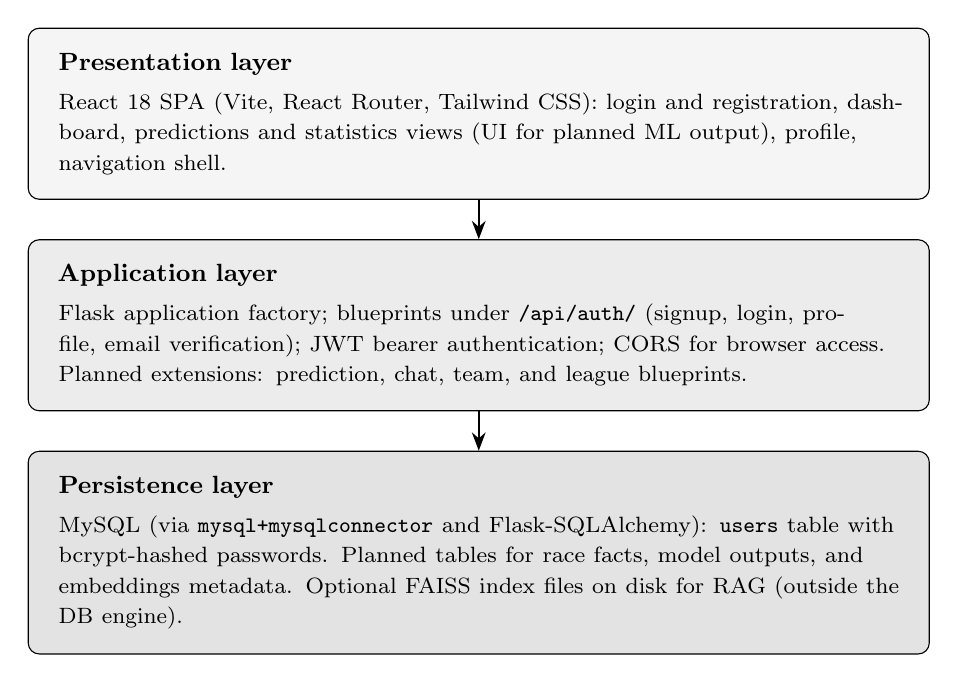
\begin{tikzpicture}[
  >=Stealth,
  font=\small,
  tier/.style={draw, rounded corners=4pt, inner xsep=11pt, inner ysep=9pt,
               align=left, anchor=north, text width=0.88\textwidth},
  arr/.style={thick, ->}
]
  \node[tier, fill=gray!8] (t1) at (0,0)
    {\textbf{Presentation layer}\\[3pt]
     {\footnotesize React~18 SPA (Vite, React Router, Tailwind~CSS): login and
     registration, dashboard, predictions and statistics views (UI for planned
     ML output), profile, navigation shell.}};
  \node[tier, fill=gray!15, below=0.5cm of t1.south] (t2)
    {\textbf{Application layer}\\[3pt]
     {\footnotesize Flask application factory; blueprints under
     \texttt{/api/auth/} (signup, login, profile, email verification); JWT
     bearer authentication; CORS for browser access. Planned extensions:
     prediction, chat, team, and league blueprints.}};
  \node[tier, fill=gray!22, below=0.5cm of t2.south] (t3)
    {\textbf{Persistence layer}\\[3pt]
     {\footnotesize MySQL (via \texttt{mysql+mysqlconnector} and Flask-SQLAlchemy):
     \texttt{users} table with bcrypt-hashed passwords. Planned tables for race
     facts, model outputs, and embeddings metadata. Optional FAISS index files
     on disk for RAG (outside the DB engine).}};
  \draw[arr] (t1.south) -- (t2.north);
  \draw[arr] (t2.south) -- (t3.north);
\end{tikzpicture}
\caption{Layered logical architecture of OVERTAKE (current vs.\ planned scope).}
\label{fig:arch}
\end{figure}

For the implemented login path, the browser sends credentials to the React
client, which POSTs JSON to \texttt{/api/auth/login}; Flask validates the user
against MySQL (bcrypt) and returns a JWT and profile payload. A future
prediction path will extend this pattern with a dedicated endpoint, feature
queries against race tables, and an attached ML inference step.

\subsection{Prediction use cases}

The prediction experience offers a \emph{default} run (fixed model behaviour) and
a \emph{user-weighted} run where the player adjusts importance weights before
inference. Figure~\ref{fig:uc-predict} captures the shared and distinct use cases
for both paths.

% Required in preamble:
% \usepackage{tikz}
% \usetikzlibrary{arrows.meta, shapes.geometric}
% \usepackage{xcolor}

\begin{figure}[H]
\centering
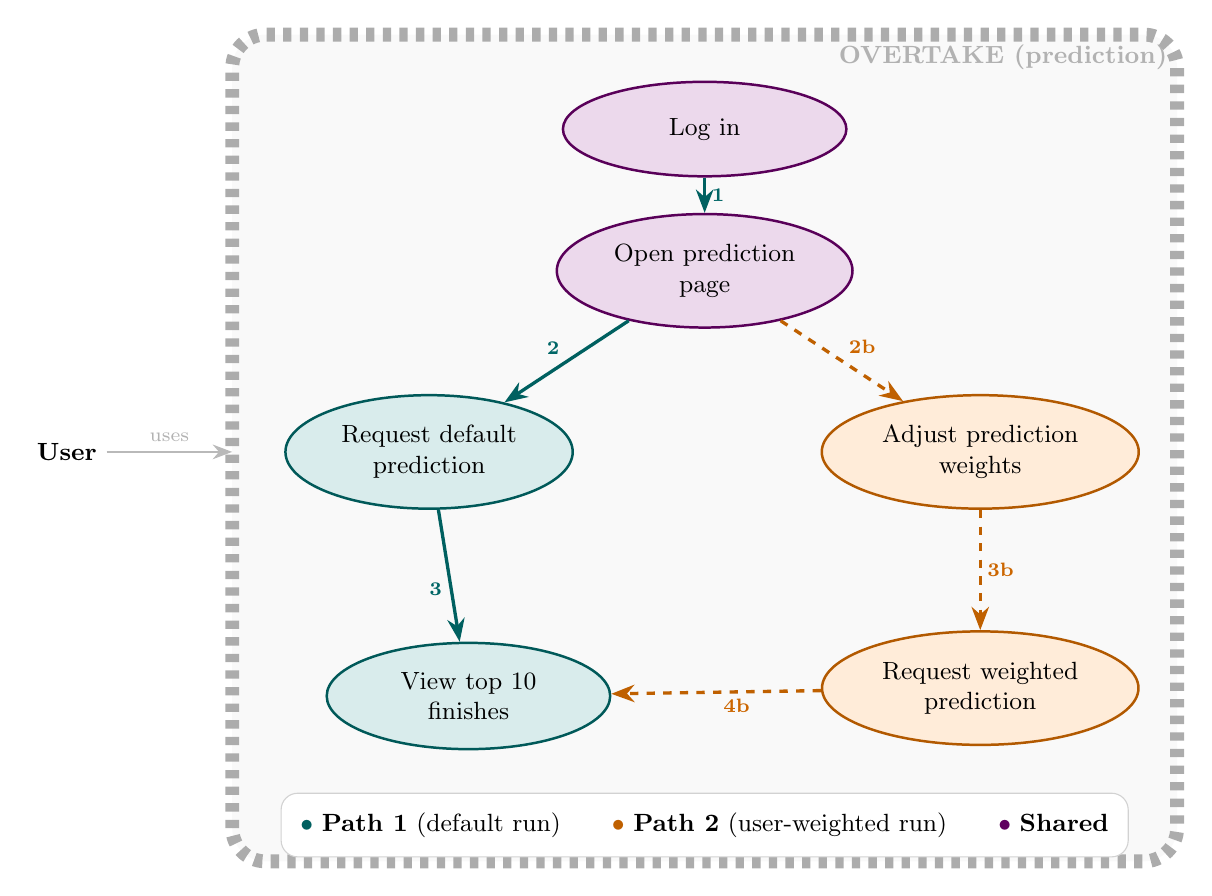
\begin{tikzpicture}[
  font=\small,
  >=Stealth,
  %--- three concrete ellipse styles, one per colour role ---
  shared/.style={
    draw=violet!70!black, fill=violet!15,
    ellipse, inner sep=5pt,
    minimum width=3.6cm, minimum height=1.2cm,
    align=center, line width=0.9pt
  },
  path1/.style={
    draw=teal!70!black, fill=teal!15,
    ellipse, inner sep=5pt,
    minimum width=3.6cm, minimum height=1.2cm,
    align=center, line width=0.9pt
  },
  path2/.style={
    draw=orange!70!black, fill=orange!15,
    ellipse, inner sep=5pt,
    minimum width=3.6cm, minimum height=1.2cm,
    align=center, line width=0.9pt
  },
  %--- arrow styles ---
  p1arr/.style={
    ->, >=Stealth,
    teal!75!black, line width=1.2pt
  },
  p2arr/.style={
    ->, >=Stealth,
    orange!75!black, line width=1.2pt, dashed
  },
  numlbl/.style={
    font=\scriptsize\bfseries, inner sep=2pt
  }
]

%------------------------------------------------------------------
%  System boundary
%------------------------------------------------------------------
\draw[draw=gray!65, fill=gray!5, dashed, rounded corners=12pt, line width=5pt]
  (0.5, 0.3) rectangle (12.5, 10.8);

\node[anchor=north east, font=\small\bfseries, text=gray!60]
  at (12.5, 10.8) {OVERTAKE (prediction)};

%------------------------------------------------------------------
%  Actor (outside boundary, centred vertically)
%------------------------------------------------------------------
\node[align=center, font=\small\bfseries] (user) at (-1.6, 5.5) {\textbf{User}};
\draw[->, gray!55, line width=0.9pt]
  (user.east) -- (0.5, 5.5)
  node[midway, above, font=\scriptsize, text=gray!60] {uses};

%------------------------------------------------------------------
%  Nodes  –  fork/join layout (top to bottom)
%
%   y=9.6   Log in                      (shared)
%   y=7.8   Open prediction page        (shared)
%   y=5.5   Req. default pred.  |  Adj. weights
%   y=3.5                       |  Req. weighted pred.
%   y=1.4   View top 10 finishes        (path1 endpoint)
%------------------------------------------------------------------

\node[shared] (login)   at (6.5, 9.6) {Log in};
\node[shared] (openpp)  at (6.5, 7.8) {Open prediction\\page};
\node[path1]  (reqdef)  at (3.0, 5.5) {Request default\\prediction};
\node[path2]  (adjwt)   at (10.0, 5.5) {Adjust prediction\\weights};
\node[path2]  (reqwt)   at (10.0, 2.5) {Request weighted\\prediction};
\node[path1]  (top10)   at (3.5, 2.4) {View top 10\\finishes};

%------------------------------------------------------------------
%  Path-1 arrows  (teal, solid)
%------------------------------------------------------------------
\draw[p1arr] (login)  -- (openpp)
  node[midway, right, numlbl, text=teal!80!black] {1};

\draw[p1arr] (openpp) -- (reqdef)
  node[midway, above left, numlbl, text=teal!80!black] {2};

\draw[p1arr] (reqdef) -- (top10)
  node[midway, below left, numlbl, text=teal!80!black] {3};

%------------------------------------------------------------------
%  Path-2 arrows  (orange, dashed)
%------------------------------------------------------------------
\draw[p2arr] (openpp) -- (adjwt)
  node[midway, above right, numlbl, text=orange!80!black] {2b};

\draw[p2arr] (adjwt)  -- (reqwt)
  node[midway, right, numlbl, text=orange!80!black] {3b};

\draw[p2arr] (reqwt)  -- (top10)
  node[midway, below right, numlbl, text=orange!80!black] {4b};

%------------------------------------------------------------------
%  Legend
%------------------------------------------------------------------
\node[draw=gray!35, fill=white, rounded corners=6pt,
      inner sep=7pt, font=\small, anchor=south]
  at (6.5, 0.35)
  {%
    \textcolor{teal!75!black}{$\bullet$}~\textbf{Path 1} (default run)\qquad
    \textcolor{orange!75!black}{$\bullet$}~\textbf{Path 2} (user-weighted run)\qquad
    \textcolor{violet!75!black}{$\bullet$}~\textbf{Shared}%
  };

\end{tikzpicture}
\caption{%
  Use cases for driver prediction.
  \textbf{Path~1} (teal):
    Log in $\to$ Open prediction page $\to$
    Request default prediction $\to$ View top~10 finishes.
  \textbf{Path~2} (orange) branches at Open prediction page:
    Adjust prediction weights $\to$
    Request weighted prediction $\to$ View top~10 finishes.
}
\label{fig:uc-predict}
\end{figure}
\subsection{Prediction interaction flows}

Figure~\ref{fig:seq-predict-paths} shows the intended HTTP-level interaction for
each path. Both assume an authenticated session; the only behavioural
difference is whether the predict request carries default parameters or a
user-supplied weight vector consumed by the model service.

%------------------------------------------------------------------
% Shared macros (put before \begin{document} or in preamble)
%------------------------------------------------------------------
% \xU=0  \xR=3.5  \xF=7.5  \xM=11.5   (lifeline x-coords)
 
\begin{figure}[H]
\centering
 
%%==============================================================
%%  PATH 1
%%==============================================================
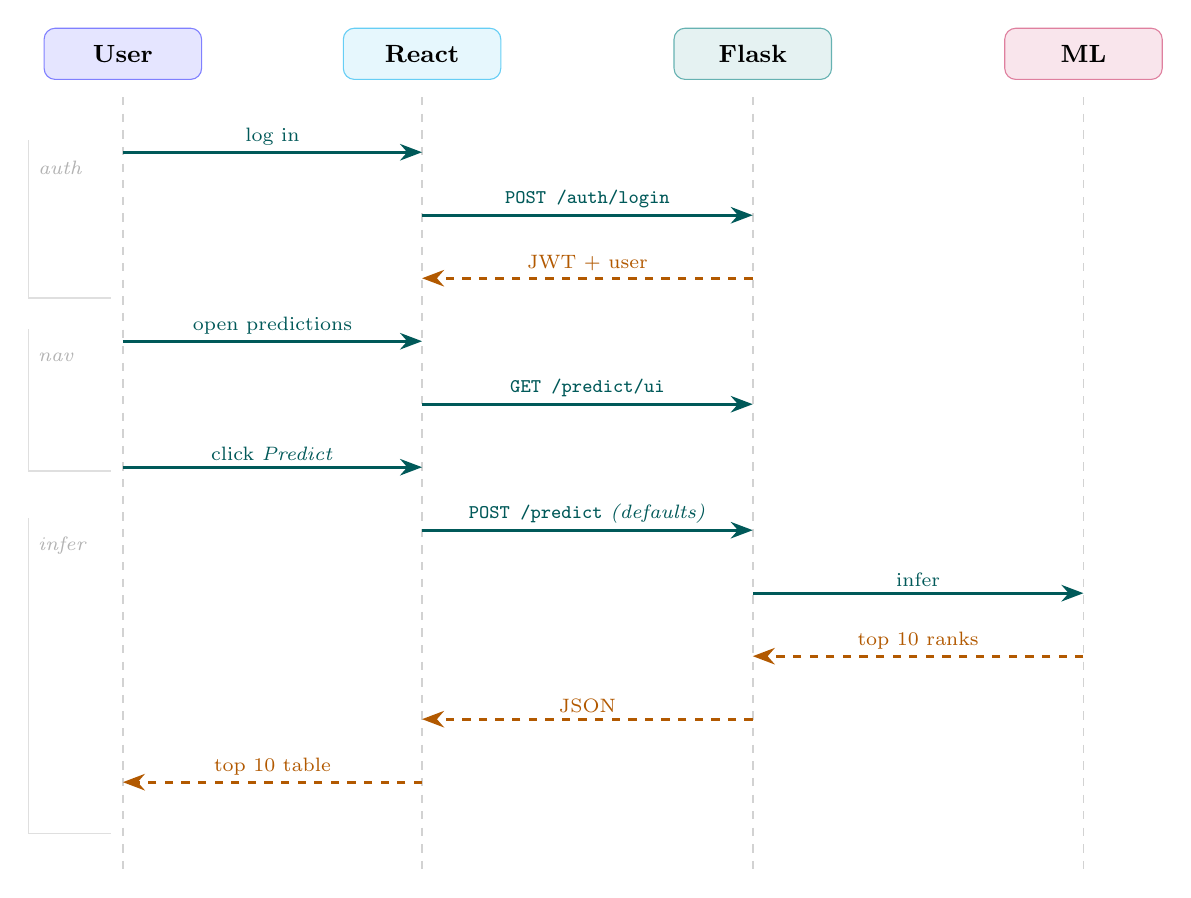
\begin{tikzpicture}[
  font=\small, >=Stealth,
  req/.style={->, >=Stealth, teal!70!black,   line width=1.1pt},
  res/.style={->, >=Stealth, orange!70!black, line width=1.1pt, dashed},
  msg/.style={font=\scriptsize, inner sep=2pt, fill=white, rounded corners=2pt}
]
  \def\xU{0}   \def\xR{3.8}  \def\xF{8.0}  \def\xM{12.2}
  \def\ytop{0} \def\ybot{-9.8}
 
  %--- lifeline headers (each with its own colour) ---
  \node[draw=blue!50,   fill=blue!10,   rounded corners=4pt,
        minimum width=2cm, minimum height=0.65cm,
        font=\small\bfseries, align=center]
    at (\xU,0.55) {User};
  \node[draw=cyan!60,   fill=cyan!10,   rounded corners=4pt,
        minimum width=2cm, minimum height=0.65cm,
        font=\small\bfseries, align=center]
    at (\xR,0.55) {React};
  \node[draw=teal!60,   fill=teal!10,   rounded corners=4pt,
        minimum width=2cm, minimum height=0.65cm,
        font=\small\bfseries, align=center]
    at (\xF,0.55) {Flask};
  \node[draw=purple!50, fill=purple!10, rounded corners=4pt,
        minimum width=2cm, minimum height=0.65cm,
        font=\small\bfseries, align=center]
    at (\xM,0.55) {ML};
 
  %--- lifelines ---
  \foreach \x in {\xU,\xR,\xF,\xM}
    \draw[dashed, gray!35, line width=0.7pt] (\x,\ytop) -- (\x,\ybot);
 
  %--- phase label: authentication ---
  \node[font=\scriptsize\itshape, text=gray!60, anchor=west]
    at (-1.2,-0.9) {auth};
  \draw[gray!25, line width=0.5pt]
    (-1.2,-0.55) -- (-1.2,-2.55) -- (-0.15,-2.55);
 
  %--- messages ---
  % 1
  \draw[req] (\xU,-0.7) -- (\xR,-0.7)
    node[midway, above, msg] {log in};
  % 2
  \draw[req] (\xR,-1.5) -- (\xF,-1.5)
    node[midway, above, msg] {\texttt{POST /auth/login}};
  % 3  (response ←)
  \draw[res] (\xF,-2.3) -- (\xR,-2.3)
    node[midway, above, msg] {JWT + user};
 
  %--- phase label: navigation ---
  \node[font=\scriptsize\itshape, text=gray!60, anchor=west]
    at (-1.2,-3.3) {nav};
  \draw[gray!25, line width=0.5pt]
    (-1.2,-2.95) -- (-1.2,-4.75) -- (-0.15,-4.75);
 
  % 4
  \draw[req] (\xU,-3.1) -- (\xR,-3.1)
    node[midway, above, msg] {open predictions};
  % 5
  \draw[req] (\xR,-3.9) -- (\xF,-3.9)
    node[midway, above, msg] {\texttt{GET /predict/ui}};
  % 6
  \draw[req] (\xU,-4.7) -- (\xR,-4.7)
    node[midway, above, msg] {click \textit{Predict}};
 
  %--- phase label: inference ---
  \node[font=\scriptsize\itshape, text=gray!60, anchor=west]
    at (-1.2,-5.7) {infer};
  \draw[gray!25, line width=0.5pt]
    (-1.2,-5.35) -- (-1.2,-9.35) -- (-0.15,-9.35);
 
  % 7
  \draw[req] (\xR,-5.5) -- (\xF,-5.5)
    node[midway, above, msg] {\texttt{POST /predict} \textit{(defaults)}};
  % 8
  \draw[req] (\xF,-6.3) -- (\xM,-6.3)
    node[midway, above, msg] {infer};
  % 9  (response ←)
  \draw[res] (\xM,-7.1) -- (\xF,-7.1)
    node[midway, above, msg] {top 10 ranks};
  % 10 (response ←)
  \draw[res] (\xF,-7.9) -- (\xR,-7.9)
    node[midway, above, msg] {JSON};
  % 11 (response ←)
  \draw[res] (\xR,-8.7) -- (\xU,-8.7)
    node[midway, above, msg] {top 10 table};
 
\end{tikzpicture}
 
\vspace{0.3cm}
{\small\textit{(a) Path 1: normal (default) prediction.}}
 
\vspace{1.2cm}
 
%%==============================================================
%%  PATH 2
%%==============================================================
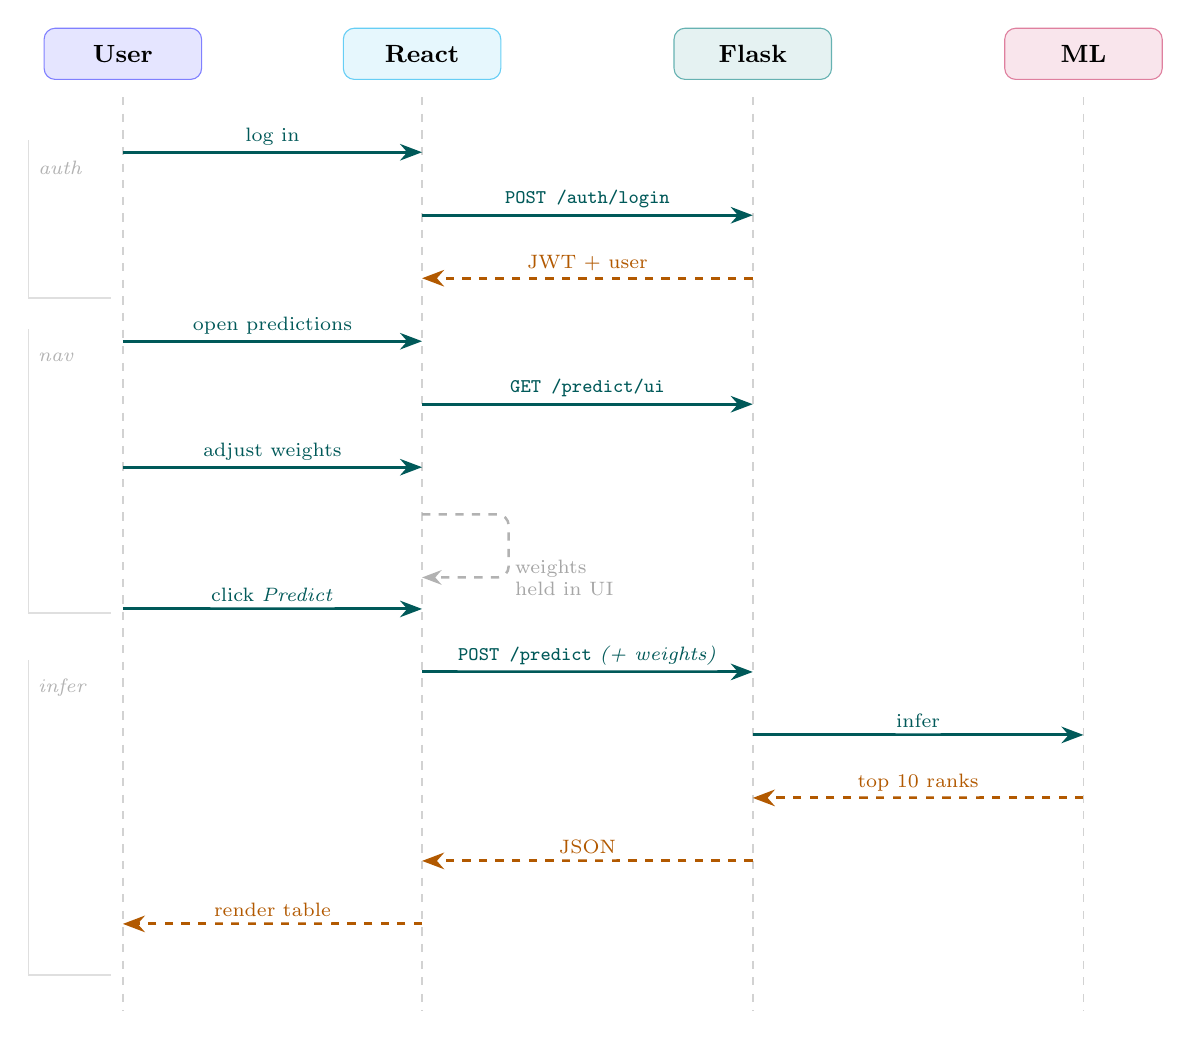
\begin{tikzpicture}[
  font=\small, >=Stealth,
  req/.style={->, >=Stealth, teal!70!black,   line width=1.1pt},
  res/.style={->, >=Stealth, orange!70!black, line width=1.1pt, dashed},
  slf/.style={->, >=Stealth, gray!60,          line width=0.9pt, dashed,
              rounded corners=4pt},
  msg/.style={font=\scriptsize, inner sep=2pt, fill=white, rounded corners=2pt}
]
  \def\xU{0}   \def\xR{3.8}  \def\xF{8.0}  \def\xM{12.2}
  \def\ytop{0} \def\ybot{-11.6}
 
  %--- lifeline headers ---
  \node[draw=blue!50,   fill=blue!10,   rounded corners=4pt,
        minimum width=2cm, minimum height=0.65cm,
        font=\small\bfseries, align=center]
    at (\xU,0.55) {User};
  \node[draw=cyan!60,   fill=cyan!10,   rounded corners=4pt,
        minimum width=2cm, minimum height=0.65cm,
        font=\small\bfseries, align=center]
    at (\xR,0.55) {React};
  \node[draw=teal!60,   fill=teal!10,   rounded corners=4pt,
        minimum width=2cm, minimum height=0.65cm,
        font=\small\bfseries, align=center]
    at (\xF,0.55) {Flask};
  \node[draw=purple!50, fill=purple!10, rounded corners=4pt,
        minimum width=2cm, minimum height=0.65cm,
        font=\small\bfseries, align=center]
    at (\xM,0.55) {ML};
 
  %--- lifelines ---
  \foreach \x in {\xU,\xR,\xF,\xM}
    \draw[dashed, gray!35, line width=0.7pt] (\x,\ytop) -- (\x,\ybot);
 
  %--- phase: auth ---
  \node[font=\scriptsize\itshape, text=gray!60, anchor=west]
    at (-1.2,-0.9) {auth};
  \draw[gray!25, line width=0.5pt]
    (-1.2,-0.55) -- (-1.2,-2.55) -- (-0.15,-2.55);
 
  \draw[req] (\xU,-0.7) -- (\xR,-0.7)
    node[midway, above, msg] {log in};
  \draw[req] (\xR,-1.5) -- (\xF,-1.5)
    node[midway, above, msg] {\texttt{POST /auth/login}};
  \draw[res] (\xF,-2.3) -- (\xR,-2.3)
    node[midway, above, msg] {JWT + user};
 
  %--- phase: navigation + weight adjustment ---
  \node[font=\scriptsize\itshape, text=gray!60, anchor=west]
    at (-1.2,-3.3) {nav};
  \draw[gray!25, line width=0.5pt]
    (-1.2,-2.95) -- (-1.2,-6.55) -- (-0.15,-6.55);
 
  \draw[req] (\xU,-3.1) -- (\xR,-3.1)
    node[midway, above, msg] {open predictions};
  \draw[req] (\xR,-3.9) -- (\xF,-3.9)
    node[midway, above, msg] {\texttt{GET /predict/ui}};
  \draw[req] (\xU,-4.7) -- (\xR,-4.7)
    node[midway, above, msg] {adjust weights};
 
  % self-arrow on React: weights held in UI
  \draw[slf] (\xR,-5.3) -- ++(1.1,0) -- ++(0,-0.8) -- (\xR,-6.1)
    node[pos=0.5, right, xshift=0.5cm, font=\scriptsize,
         text=gray!70, align=left] {weights\\held in UI};
 
  \draw[req] (\xU,-6.5) -- (\xR,-6.5)
    node[midway, above, msg] {click \textit{Predict}};
 
  %--- phase: inference ---
  \node[font=\scriptsize\itshape, text=gray!60, anchor=west]
    at (-1.2,-7.5) {infer};
  \draw[gray!25, line width=0.5pt]
    (-1.2,-7.15) -- (-1.2,-11.15) -- (-0.15,-11.15);
 
  \draw[req] (\xR,-7.3) -- (\xF,-7.3)
    node[midway, above, msg] {\texttt{POST /predict} \textit{(+ weights)}};
  \draw[req] (\xF,-8.1) -- (\xM,-8.1)
    node[midway, above, msg] {infer};
  \draw[res] (\xM,-8.9) -- (\xF,-8.9)
    node[midway, above, msg] {top 10 ranks};
  \draw[res] (\xF,-9.7) -- (\xR,-9.7)
    node[midway, above, msg] {JSON};
  \draw[res] (\xR,-10.5) -- (\xU,-10.5)
    node[midway, above, msg] {render table};
 
\end{tikzpicture}
 
\vspace{0.3cm}
{\small\textit{(b) Path 2: user-weighted prediction.}}
 
\vspace{0.6cm}
 
% legend
\noindent
\hfill
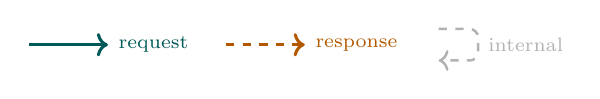
\begin{tikzpicture}[font=\scriptsize, baseline]
  \draw[->, teal!70!black,   line width=1.1pt]        (0,0) -- (1,0)
    node[right] {request};
  \draw[->, orange!70!black, line width=1.1pt, dashed] (2.5,0) -- (3.5,0)
    node[right] {response};
  \draw[->, gray!60,         line width=0.9pt, dashed,
        rounded corners=3pt]                           (5.2,0.2) -- ++(0.5,0)
    -- ++(0,-0.4) -- ++(-0.5,0)
    node[right, xshift=0.5cm, yshift=0.2cm] {internal};
\end{tikzpicture}
\hfill\strut
 
\caption{Interaction diagrams for the two prediction paths.
  Endpoint names are illustrative and will match the Flask blueprint once exposed.}
\label{fig:seq-predict-paths}
\end{figure}
\section{Database Design}

\textbf{MySQL} was selected for relational modelling of users and, in later
iterations, normalised race and prediction entities. A relational design supports
foreign keys, transactional consistency for sign-up and league updates, and
straightforward reporting queries compared to a schemaless store for these
workloads. The current and planned principal tables include:

\begin{itemize}[leftmargin=*]
  \item \texttt{users} --- primary key, name, unique email, bcrypt password hash,
        optional age, timestamps (implemented).
  \item \texttt{races}, \texttt{sessions}, \texttt{results} --- normalised race
        and session facts derived from FastF1 (planned).
  \item \texttt{predictions} --- model outputs keyed by race and driver (planned).
  \item \texttt{teams}, \texttt{leagues}, \texttt{league\_members} --- fantasy
        constructs and scores (planned).
  \item \texttt{documents} / file-backed FAISS --- chunk metadata for RAG
        (planned; vector index may live outside MySQL).
\end{itemize}

\section{Machine Learning Pipeline}
\label{sec:ml-pipeline}

The end-to-end machine learning pipeline covers the following stages:
\[
\text{Raw Data (FastF1)} \;\rightarrow\;
\text{Feature Engineering} \;\rightarrow\;
\text{Rolling Training} \;\rightarrow\;
\text{Three-Model Ensemble} \;\rightarrow\;
\text{Rank Aggregation} \;\rightarrow\;
\text{Predicted Finishing Order}
\]

Race data for seasons 2022--2025 is ingested via the FastF1 Python library, covering
lap times, telemetry, qualifying results, practice sessions, race results, race-control
messages, and weather readings. Feature engineering is applied per driver per race
weekend, producing a flat feature matrix of 73 engineered signals stored in a Parquet
file (\texttt{f1\_features.parquet}) that is recomputed after every new race. The
model is evaluated with a rolling-forward validation protocol on the 2025 season: for
each race round $r$, all models are trained exclusively on data from rounds prior to
$r$ across all available seasons, then used to predict round $r$. This strictly
respects temporal ordering and prevents any form of data leakage.

\subsection{Target Variable}
\label{subsec:target}

Rather than classifying binary outcomes, the primary regression target is the
natural-logarithm-transformed finishing position:
\[
\text{LogPosition} = \ln(1 + \text{FinalPosition})
\]
Log-transformation compresses the upper tail of positions 11--20 (where ordering
matters less for fantasy scoring) and gives proportionally greater weight to
front-of-field accuracy. Drivers who did not finish (DNF) are assigned a worst-case
position of 20 before transformation, equivalent to $\ln(21) \approx 3.04$.

\subsection{Feature Engineering}
\label{subsec:features}

Seventy-three pre-race features are derived from session data and divided into twelve
categories. Every rolling-window statistic is shifted by one race to prevent leakage
(i.e., the value for race $r$ reflects races up to $r-1$ only). Missing values are
imputed with the sentinel value $-999$, allowing gradient-boosted trees to route
missing entries down a dedicated branch rather than applying mean imputation.

\begin{table}[H]
\centering
\caption{Complete feature set for the ML predictor (73 features across 12 categories).}
\label{tab:features}
\renewcommand{\arraystretch}{1.2}
\begin{tabularx}{\textwidth}{@{} l l X @{}}
  \toprule
  \textbf{Category} & \textbf{Feature(s)} & \textbf{Description} \\
  \midrule
  \multirow{4}{*}{Qualifying}
    & \texttt{QualiPosition}, \texttt{QualiStage}
      & Final qualifying classification and furthest session reached (Q1/Q2/Q3). \\
    & \texttt{BestQualiTime\_sec}
      & Best lap time in the qualifying session (seconds). \\
    & \texttt{GapToPole\_sec}, \texttt{GapToPole\_pct}
      & Absolute and percentage gap to pole-position time. \\
    & \texttt{Q1\_sec}, \texttt{Q2\_sec}, \texttt{Q3\_sec}
      & Individual-session lap times (NaN if eliminated earlier). \\
  \midrule
  \multirow{5}{*}{Practice sessions}
    & \texttt{P1/P2/P3\_BestLap\_sec}
      & Best recorded lap time in each practice session. \\
    & \texttt{P1/P2/P3\_GapToFastest\_sec}
      & Gap to the fastest driver in the same session. \\
    & \texttt{P2\_LongRunMean/Median/Laps/Gap\_sec}
      & P2 long-stint proxy: mean and median pace over laps $\geq 2$ in a stint, run length, and gap to fastest long-run. \\
    & \texttt{P3\_GapS1/S2/S3\_sec}
      & P3 per-sector gap to the fastest sector time. \\
    & \texttt{P3\_MaxSpeed}, \texttt{P3\_TrapSpeed}, \texttt{P3\_S1/S2/S3\_frac}
      & Maximum and speed-trap speed; fractional sector-time contributions in P3. \\
  \midrule
  \multirow{4}{*}{Driver form}
    & \texttt{Drv\_AvgPos\_L3/L5/L10}
      & Rolling average finishing position over the last 3, 5, and 10 races. \\
    & \texttt{Drv\_AvgPos\_EWM}, \texttt{Drv\_AvgPts\_L5}, \texttt{Drv\_AvgPts\_EWM}
      & Exponentially weighted average position (half-life 4); rolling and EWM points. \\
    & \texttt{Drv\_DNFRate\_L10}, \texttt{Drv\_StdPos\_L5}
      & Historical DNF rate and finishing-position variability. \\
    & \texttt{Drv\_AvgGridDelta\_L5}
      & Average grid-to-finish position gain or loss over the last 5 races. \\
  \midrule
  \multirow{2}{*}{Season standing}
    & \texttt{Drv\_SeasonPts\_cumulative}, \texttt{Drv\_SeasonRaceCount}
      & Cumulative points in the current season (excluding current race); races completed so far. \\
    & \texttt{SeasonCumPts}, \texttt{PtsGapToLeader}, \texttt{ChampionshipRank}
      & Season total, points gap to championship leader, and current championship rank. \\
  \midrule
  \multirow{3}{*}{Team history}
    & \texttt{Team\_AvgPos\_L5}, \texttt{Team\_AvgPos\_EWM}
      & Team's rolling and EWM average finishing position. \\
    & \texttt{Team\_AvgPts\_L5}, \texttt{Team\_DNFRate\_L10}
      & Team points trend and recent DNF rate. \\
    & \texttt{Team\_SeasonPts\_cumulative}
      & Team's cumulative season points (excluding current race). \\
  \midrule
  \multirow{3}{*}{Circuit history}
    & \texttt{Drv\_CircuitAvgPos}, \texttt{Drv\_CircuitAvgPts}
      & Driver's historical average position and points at this specific circuit. \\
    & \texttt{Drv\_CircuitDNFRate}, \texttt{Drv\_CircuitRaceCount}
      & Historical DNF rate and number of starts at this circuit. \\
    & \texttt{Drv\_CircuitGridDelta}
      & Average grid-to-finish delta at this circuit (global average for debut visit). \\
  \midrule
  Elo rating
    & \texttt{Elo\_before}, \texttt{Elo\_rank}
      & Elo rating before the race (pairwise updates from classified finishers; DNFs excluded) and within-grid rank of that rating. \\
  \midrule
  \multirow{2}{*}{Weekend meta}
    & \texttt{IsSprintWeekend}, \texttt{IsStreetCircuit}
      & Binary flags for sprint-format weekends and street circuits (Monaco, Singapore, Baku, etc.). \\
    & \texttt{SeasonProgress}
      & Fractional round index in $[0,1]$ indicating how far through the season the race falls. \\
  \midrule
  \multirow{2}{*}{Circuit chaos}
    & \texttt{Circuit\_AvgSC\_hist}, \texttt{Circuit\_AvgFlags\_hist}
      & Historical mean safety-car count and yellow-flag count at this circuit. \\
    & \texttt{Circuit\_HistChaos}, \texttt{Circuit\_HistUpsetRate}
      & Historical std of grid-to-finish deltas; fraction of drivers who moved more than 5 places from grid. \\
  \midrule
  \multirow{2}{*}{Recent form}
    & \texttt{Form\_Pts\_L3}, \texttt{Form\_PodiumRate\_L5}
      & Average points in the last 3 races; podium frequency over the last 5. \\
    & \texttt{Form\_InPointsRate\_L5}, \texttt{Form\_ConsecDNF}
      & Top-10 finish rate over 5 races; consecutive-race DNF count (rolling window 3). \\
  \midrule
  Teammate
    & \texttt{Tm\_BeatRate\_L5}, \texttt{Tm\_QualiGap\_EWM}, \texttt{Tm\_PosGap\_EWM}
      & Rate of outfinishing the team-mate over the last 5 shared races; EWM qualifying and finishing position gap relative to team-mate. \\
  \midrule
  \multirow{2}{*}{Weather}
    & \texttt{Wx\_AvgAirTemp}, \texttt{Wx\_AvgTrackTemp}, \texttt{Wx\_AvgHumidity}
      & Race-session average air temperature, track temperature, and humidity. \\
    & \texttt{Wx\_AvgWindSpeed}, \texttt{Wx\_RainfallFrac}, \texttt{Wx\_AnyRain}, \texttt{Wx\_TrackTempSpread}
      & Average wind speed; fraction of readings with rainfall; binary rain indicator; range of track temperature across the session. \\
  \bottomrule
\end{tabularx}
\end{table}

\subsection{Model Architecture: Three-Model Ensemble}
\label{subsec:model-arch}

Three independently trained models produce per-driver scores that are combined
into a single \emph{Combined Score}, which is ranked to determine the predicted
finishing order. Each component score is min-max normalised to $[0,1]$ within
the race grid before combination.

\subsubsection*{Model 1 --- LightGBM Position Regressor}

A \texttt{LGBMRegressor} is trained on all 73 features to predict \texttt{LogPosition}
using mean-squared-error loss. Early stopping (patience 50~rounds) is applied
against an internal validation set comprising the most recent calendar year in
the training window, preventing overfitting as training data accumulates round
by round.

\begin{table}[H]
\centering
\caption{LightGBM position regressor hyperparameters.}
\label{tab:lgbm-hparams}
\begin{tabular}{@{} l r @{}}
  \toprule
  \textbf{Hyperparameter} & \textbf{Value} \\
  \midrule
  \texttt{n\_estimators}       & 600 \\
  \texttt{learning\_rate}      & 0.02 \\
  \texttt{max\_depth}          & 6 \\
  \texttt{num\_leaves}         & 63 \\
  \texttt{min\_child\_samples} & 10 \\
  \texttt{subsample}           & 0.8 \\
  \texttt{colsample\_bytree}   & 0.7 \\
  \texttt{reg\_alpha}          & 0.1 \\
  \texttt{reg\_lambda}         & 0.1 \\
  \texttt{random\_state}       & 42 \\
  \bottomrule
\end{tabular}
\end{table}

The normalised position score $\text{Score\_Pos}_i \in [0,1]$ is derived from
the raw prediction $\hat{y}_i$ where a lower value indicates a better predicted
position:
\[
\text{Score\_Pos}_i = \frac{\hat{y}_i - \min_j \hat{y}_j}{\max_j \hat{y}_j - \min_j \hat{y}_j + \varepsilon}
\]

\subsubsection*{Model 2 --- XGBoost Pairwise Ranker}

An \texttt{XGBRanker} with \texttt{objective=rank:pairwise} is trained on all
races in the training window simultaneously. Labels are inverted
($\text{label} = P_{\max}+1-\text{FinalPosition}$) so that higher relevance
corresponds to a better finish. Groups are defined by (Season,~RoundNumber)
tuples. Key hyperparameters: \texttt{n\_estimators=400},
\texttt{learning\_rate=0.05}, \texttt{max\_depth=5},
\texttt{eval\_metric=ndcg@10}. The normalised, inverted rank score
$\text{Score\_Rank}_i \in [0,1]$ is computed analogously.

\subsubsection*{Model 3 --- Calibrated LightGBM DNF Classifier}

A \texttt{LGBMClassifier} trained on 12 DNF-specific features (driver and team
DNF rates, circuit-specific DNF rate, consecutive-DNF count, weather indicators,
sprint-weekend flag, and Elo rating) predicts the binary DNF outcome. Class
imbalance is handled via \texttt{scale\_pos\_weight}. Probability calibration is
applied via \texttt{CalibratedClassifierCV} to ensure that predicted
probabilities reflect true historical DNF frequencies. The classifier outputs
$\text{DNF\_Prob}_i \in [0,1]$.

\subsection{Ensemble Score Combination}
\label{subsec:ensemble}

The three normalised scores are combined using dynamically adjusted weights:
\[
\text{Combined\_Score}_i =
  w_{\text{pos}} \cdot \text{Score\_Pos}_i
  + w_{\text{rank}} \cdot \text{Score\_Rank}_i
  + w_{\text{dnf}} \cdot \text{DNF\_Prob}_i
\]

Weights are a function of season progress $p \in [0,1]$ and circuit type:
\begin{align*}
  w_{\text{rank}} &= 0.40 + 0.15\,(1-p) \\
  w_{\text{pos}}  &= 0.40 - 0.10\,(1-p) \\
  w_{\text{dnf}}  &=
    \begin{cases}
      0.30 & \text{street circuit (Monaco, Singapore, Baku, etc.)} \\
      0.22 & \text{permanent circuit}
    \end{cases}
\end{align*}

All three weights are re-normalised to sum to 1 after computation. Early in
the season ($p \approx 0$) rolling features are sparse, so the ranker --- which
uses all available historical seasons rather than only recent windows --- receives
more weight. As the season progresses and per-season rolling statistics become
richer, the position regressor gains proportionally more influence.
Figure~\ref{fig:ensemble-weights} illustrates the weight evolution over a 24-round
season for a permanent circuit.

\begin{figure}[H]
\centering
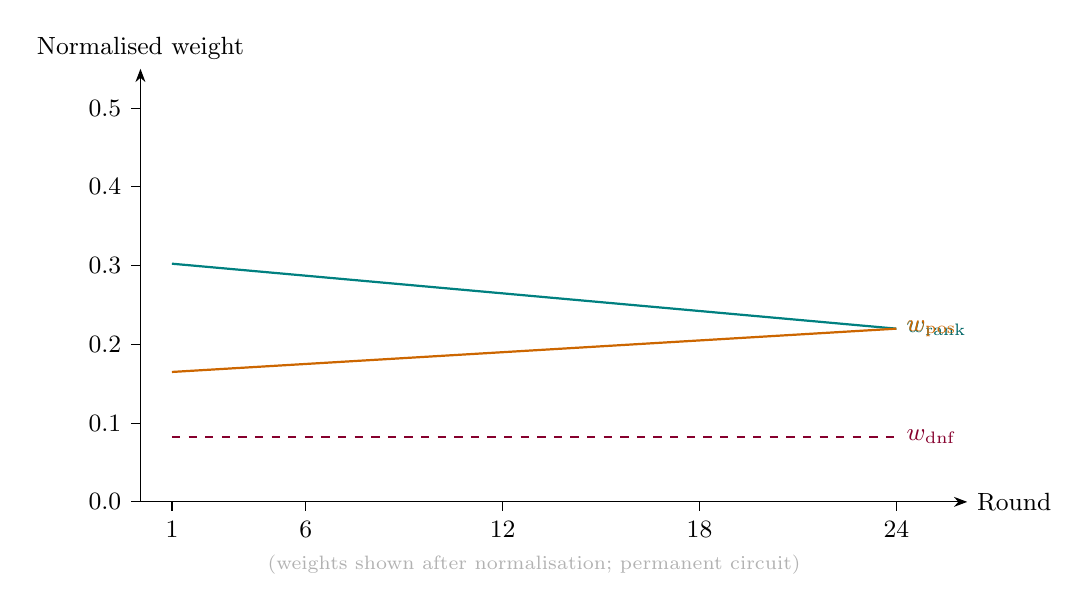
\begin{tikzpicture}[font=\small, >=Stealth]
  \draw[->] (0,0) -- (10.5,0) node[right] {Round};
  \draw[->] (0,0) -- (0,5.5)  node[above] {Normalised weight};

  % tick marks and labels on x-axis (rounds 1, 6, 12, 18, 24)
  \foreach \r/\x in {1/0.4, 6/2.1, 12/4.6, 18/7.1, 24/9.6} {
    \draw (\x,0) -- (\x,-0.12) node[below] {\r};
  }
  % y-axis ticks 0.1 ... 0.6
  \foreach \y/\yv in {0/0.0,1/0.1,2/0.2,3/0.3,4/0.4,5/0.5} {
    \draw (0,\y) -- (-0.12,\y) node[left] {\yv};
  }

  % w_rank: starts high, decreases (0.55 -> 0.40)
  \draw[teal, thick]
    (0.4,5.5*0.55) -- (9.6,5.5*0.40)
    node[right, text=teal!80!black] {$w_\text{rank}$};

  % w_pos: starts lower, increases (0.30 -> 0.40)
  \draw[orange!80!black, thick]
    (0.4,5.5*0.30) -- (9.6,5.5*0.40)
    node[right, text=orange!80!black] {$w_\text{pos}$};

  % w_dnf: flat (0.22, renorm ~0.15)
  \draw[purple!70!black, thick, dashed]
    (0.4,5.5*0.15) -- (9.6,5.5*0.15)
    node[right, text=purple!70!black] {$w_\text{dnf}$};

  \node[font=\scriptsize, text=gray!60] at (5, -0.8)
    {(weights shown after normalisation; permanent circuit)};
\end{tikzpicture}
\caption{Dynamic ensemble weight evolution across a 24-round season (permanent circuit).
  The ranker weight decreases as rolling in-season features become richer;
  the position-regressor weight increases correspondingly.}
\label{fig:ensemble-weights}
\end{figure}

\subsection{Post-Score Adjustments}
\label{subsec:adjustments}

Two circuit-aware corrections are applied to \texttt{Combined\_Score} before
final ranking.

\paragraph{Grid penalty correction.}
When a driver's actual grid position exceeds their qualifying classification by
more than two places (indicating a regulatory or engine-mode grid penalty), a
normalised additive correction is applied:
\[
\text{Combined\_Score}_i \;\mathrel{+}=\;
  0.12 \times
  \frac{\max\bigl(0,\,\text{GridPos}_i - \text{QualiPos}_i\bigr)}%
       {\max_j\bigl(\text{GridPos}_j - \text{QualiPos}_j\bigr)}
\]
This correctly pushes pit-lane starters and penalised drivers toward the back
of the predicted order.

\paragraph{Circuit chaos blend.}
On circuits with a high historical standard deviation of grid-to-finish position
changes (\texttt{Circuit\_HistChaos}), predictions are blended toward simple
grid order:
\[
\text{Combined\_Score}_i \;\leftarrow\;
  (1-\alpha)\,\text{Combined\_Score}_i + \alpha\,\text{GridNorm}_i,
  \qquad
  \alpha = \min\!\left(\frac{\texttt{Circuit\_HistChaos}}{8},\,1\right)\times 0.35
\]
where $\text{GridNorm}_i \in [0,1]$ is the min-max normalised grid position.
The maximum blend of 35\% is applied when $\texttt{Circuit\_HistChaos} \geq 8$.

\subsection{User-Adjustable Insight Weights}
\label{subsec:user-weights}

An optional post-prediction blending layer gives fantasy players agency over
which factors they trust most. Five user-specified weights $w_k \in [0,10]$
cover the categories \emph{Driver Skill}, \emph{Team Performance},
\emph{Track History}, \emph{Weather Condition}, and \emph{Recent Form}.
For each category, a normalised per-driver score $c_{ik} \in [0,1]$ is computed
from the underlying feature values using min-max normalisation (where 0~represents
the best outcome for that category).

The blend is activated \emph{only} when weights are unequal; setting all weights
to any uniform value (e.g., all~5 or all~0) returns the pure model output
unchanged. Blend strength is driven by the standard deviation of the user weights:
\[
\alpha_{\text{user}} = \frac{\sigma(\{w_k\})}{4.9} \times 0.50
\]
where 4.9 is the theoretical maximum standard deviation for five values in
$[0,10]$. The blended final score is:
\[
\text{FinalScore}_i =
  (1-\alpha_{\text{user}})\,\widetilde{\text{Combined}}_i
  + \alpha_{\text{user}}\sum_{k} \frac{w_k}{\sum_l w_l}\,c_{ik}
\]
where $\widetilde{\text{Combined}}_i$ is the min-max normalised Combined Score.
At maximum divergence ($\sigma \approx 4.9$), the user signal accounts for up to
50\% of the final ranking; in practice, moderate weight divergence (e.g.,
$\sigma \approx 2$) applies roughly a 20\% user signal. This design ensures that
\emph{preferences} rather than absolute magnitudes determine the influence.

\subsection{Training Protocol and Data Scale}
\label{subsec:training}

\paragraph{Rolling-forward validation.}
For each 2025 race round $r$:
\begin{enumerate}[leftmargin=*]
  \item All driver-race rows where (Season $< 2025$) \textbf{or}
        (Season $= 2025$ and Round $< r$) form the training set.
  \item The most recent calendar year within the training set is withheld as
        an internal validation fold for LightGBM early stopping.
  \item All three models are retrained from scratch on the training set.
  \item Pre-race features for round $r$ are assembled and passed to the
        ensemble; no future information is used.
\end{enumerate}

\paragraph{Dataset scale.}
The initial training window (before any 2025 data) comprises 1\,359 driver-race
observations spanning the 2022--2024 seasons. By the end of the 2025 season the
training window expands to approximately 1\,818 rows. With 20 drivers per race
and 24 rounds, each within-season fold adds approximately 480 new observations.

\section{RAG Chatbot Design}

The RAG retrieval path is: \textbf{user query} $\rightarrow$ \textbf{embedding}
$\rightarrow$ \textbf{vector search} over the indexed corpus $\rightarrow$
\textbf{top-$k$ chunks} concatenated with a system prompt $\rightarrow$
\textbf{LLM generation} $\rightarrow$ \textbf{answer} returned to the client
(offline chunking and index construction are performed beforehand).

The RAG pipeline follows the approach of Lewis et al.~\cite{lewisRAG2020}.
Race documents are chunked, embedded using a sentence-transformer model, and
stored in a vector index (FAISS). At inference time, the top-$k$ retrieved
chunks are prepended to the LLM prompt alongside the user query. The open-source
LLM (e.g., Mistral 7B or LLaMA 3) generates a grounded response. Prediction
outputs from the ML module are also formatted as structured text documents and
indexed, so that the chatbot can reference them when asked for explanations.

\section{API Design}

The Flask application groups routes in blueprints. JSON is used for request and
response bodies; errors return appropriate HTTP status codes. Table~\ref{tab:api}
separates \emph{implemented} authentication endpoints from routes reserved for
the predictor, chatbot, team, and league modules described elsewhere in this
report.

\begin{table}[H]
\centering
\caption{API endpoints (implemented vs.\ planned).}
\label{tab:api}
\begin{tabularx}{\textwidth}{@{} l l X @{}}
  \toprule
  \textbf{Method} & \textbf{Endpoint} & \textbf{Description} \\
  \midrule
  POST & \texttt{/api/auth/signup}   & Register user; returns JWT and user profile. \\
  POST & \texttt{/api/auth/login}    & Authenticate; returns JWT and user profile. \\
  GET  & \texttt{/api/auth/profile} & Return current user (JWT required). \\
  POST & \texttt{/api/auth/verify-email} & Check whether an email is already registered. \\
  \midrule
  GET  & \texttt{/api/predict/\{race\_id\}} & Fetch predictions (planned). \\
  POST & \texttt{/api/chat}          & Chatbot turn (planned). \\
  GET/POST & \texttt{/api/team...}   & Team CRUD (planned). \\
  GET/POST & \texttt{/api/league...} & League operations (planned). \\
  \bottomrule
\end{tabularx}
\end{table}

\section{Frontend Design}

The client is a React.js application built with Vite for fast development builds,
React Router for navigation, and Tailwind~CSS (with Radix UI primitives where
appropriate) for layout and styling. The frontend is structured around the
following views:

\begin{enumerate}[leftmargin=*]
  \item \textbf{Dashboard} --- Next-race countdown, top predictor picks, and
        recent news summaries.
  \item \textbf{Team Builder} --- Drag-and-drop driver and constructor selection
        with live budget tracking.
  \item \textbf{Predictions} --- Probability charts per driver, with a
        feature-importance panel explaining key factors.
  \item \textbf{Chatbot} --- Full-screen conversational interface with
        conversation history.
  \item \textbf{League} --- Leaderboard table with weekly score breakdowns.
\end{enumerate}

% ============================================================
\chapter{Implementation}
% ============================================================

\section{Technology Stack}

Table~\ref{tab:stack} summarises the technologies used in the implementation.

\begin{table}[H]
\centering
\caption{Technology stack.}
\label{tab:stack}
\begin{tabularx}{\textwidth}{@{} l l X @{}}
  \toprule
  \textbf{Layer}        & \textbf{Technology}   & \textbf{Rationale} \\
  \midrule
  Frontend              & React 18, Vite, Tailwind & Component model, fast HMR, utility-first styling. \\
  Backend               & Flask (Python)        & Simple routing, blueprints, wide documentation; fits course scope. \\
  ORM / DB driver       & Flask-SQLAlchemy, mysql-connector & Portable SQL, migrations path, native MySQL driver. \\
  Database              & MySQL 8.x             & ACID transactions, constraints, strong tooling for relational data. \\
  ML                    & LightGBM 4.x, XGBoost 2.x & Three-model ensemble: \texttt{LGBMRegressor} (position), \texttt{XGBRanker} (pairwise ranking), and calibrated \texttt{LGBMClassifier} (DNF probability). 73-feature pipeline implemented. \\
  Vector store          & FAISS                 & Fast approximate nearest-neighbour search (planned RAG). \\
  Embeddings            & \texttt{sentence-transformers} & Lightweight open-source encoders (planned). \\
  LLM                   & Mistral 7B (GGUF)     & Open weights; local inference via \texttt{llama-cpp-python} (planned). \\
  Authentication        & JWT + bcrypt          & Stateless API auth; salted password hashing. \\
  Data ingestion        & FastF1                & Direct access to F1 timing/telemetry for feature pipelines. \\
  Deployment            & Docker (optional)     & Reproducible multi-service setup when containerised. \\
  \bottomrule
\end{tabularx}
\end{table}

\section{Data Ingestion}

Race data for model training is fetched using the FastF1 Python
library~\cite{fastF1}, which provides a high-level interface to Formula~1 timing,
telemetry, and session results. The feature engineering module (\texttt{f1\_feature\_engineering.py})
processes all available season data (2022--2025) through a DuckDB in-process database,
producing a 73-feature Parquet file (\texttt{f1\_features.parquet}) consumed directly by
the training pipeline. This project does \emph{not} depend on the legacy Ergast HTTP API.
For the web application, a schedulable ingestion job (cron or CI-triggered) will load
new race weekends into MySQL relational tables for RAG indexing and live prediction serving.

\subsection{Data Cleaning}

Raw FastF1 data contains missing values for laps affected by red flags, safety
cars, and virtual safety cars. The following pre-processing steps are applied:

\begin{itemize}[leftmargin=*]
  \item Laps with \texttt{TrackStatus} $\neq$ \texttt{1} (green flag) are
        flagged and excluded from lap-time features.
  \item DNFs are inferred from the session result status codes and stored as a
        Boolean field.
  \item Qualifying deltas are computed relative to the session's fastest time;
        absent qualifying times (e.g., grid penalties) are imputed with the
        session median.
\end{itemize}

\section{Machine Learning Implementation}
\label{sec:ml-impl}

This section details the concrete implementation of the three-model ensemble
described in the design chapter. All model code resides in
\texttt{f1\_model.py}; feature construction is handled by
\texttt{f1\_feature\_engineering.py}, which writes the 73-column feature matrix
to \texttt{f1\_features.parquet}.

\subsection{Feature Matrix Construction}
\label{subsec:feat-matrix}

The feature engineering module queries a DuckDB in-process database that is
populated from FastF1 session exports. For each race weekend it computes every
feature listed in Table~\ref{tab:features}: qualifying metrics, practice
telemetry, rolling driver and team averages (L3 / L5 / L10 windows),
exponentially weighted moving averages (half-life 4~races), circuit-specific
history, Elo ratings, weekend-type flags, circuit chaos indices, championship
standing, teammate differentials, and weather summaries. All rolling windows are
shifted by one race to guarantee no leakage. The resulting DataFrame is written
to Parquet for fast, reproducible model training and prediction.

\subsection{Model Training}
\label{subsec:model-training}

\paragraph{LightGBM position regressor.}
Training follows the rolling-forward protocol described in
Section~\ref{subsec:training}. The most recent calendar year in the training
set is held out as a validation fold for early stopping:

\begin{lstlisting}[language=Python,
  caption={LightGBM position regressor training (simplified).}]
from lightgbm import LGBMRegressor

model_pos = LGBMRegressor(
    n_estimators=600, learning_rate=0.02,
    max_depth=6, num_leaves=63,
    min_child_samples=10, subsample=0.8,
    colsample_bytree=0.7, reg_alpha=0.1,
    reg_lambda=0.1, random_state=42,
    n_jobs=-1
)
model_pos.fit(
    X_train, y_train,          # LogPosition target
    eval_set=[(X_val, y_val)],
    callbacks=[early_stopping(50, verbose=False),
               log_evaluation(period=-1)]
)
\end{lstlisting}

\paragraph{XGBoost pairwise ranker.}
Groups are defined per (Season, RoundNumber). Finishing-position labels are
inverted so that relevance scores are highest for race winners:

\begin{lstlisting}[language=Python,
  caption={XGBoost pairwise ranker training (simplified).}]
from xgboost import XGBRanker

model_rank = XGBRanker(
    objective='rank:pairwise', eval_metric='ndcg@10',
    n_estimators=400, learning_rate=0.05,
    max_depth=5, subsample=0.8,
    colsample_bytree=0.7, random_state=42
)
model_rank.fit(
    X_train, rank_labels,
    group=group_sizes,
    eval_set=[(X_val, rank_labels_val)],
    eval_group=[val_group_sizes],
    verbose=False
)
\end{lstlisting}

\paragraph{Calibrated LightGBM DNF classifier.}
A \texttt{LGBMClassifier} is trained on 12 DNF-specific features.
\texttt{CalibratedClassifierCV} with \texttt{cv='prefit'} applies isotonic
regression on the held-out validation fold to correct overconfident probability
estimates:

\begin{lstlisting}[language=Python,
  caption={Calibrated DNF classifier training (simplified).}]
from lightgbm import LGBMClassifier
from sklearn.calibration import CalibratedClassifierCV

base_clf = LGBMClassifier(
    n_estimators=300, learning_rate=0.05,
    max_depth=5, scale_pos_weight=neg/pos,
    random_state=42, n_jobs=-1
)
base_clf.fit(X_train_dnf, y_train_dnf,
             eval_set=[(X_val_dnf, y_val_dnf)],
             callbacks=[early_stopping(30, verbose=False)])

model_dnf = CalibratedClassifierCV(base_clf, cv='prefit',
                                    method='isotonic')
model_dnf.fit(X_val_dnf, y_val_dnf)
\end{lstlisting}

\subsection{Ensemble Prediction and Ranking}
\label{subsec:ensemble-impl}

At prediction time, the three trained models score each driver independently.
Algorithm~\ref{alg:ensemble} shows the complete inference procedure.

\begin{figure}[H]
\centering
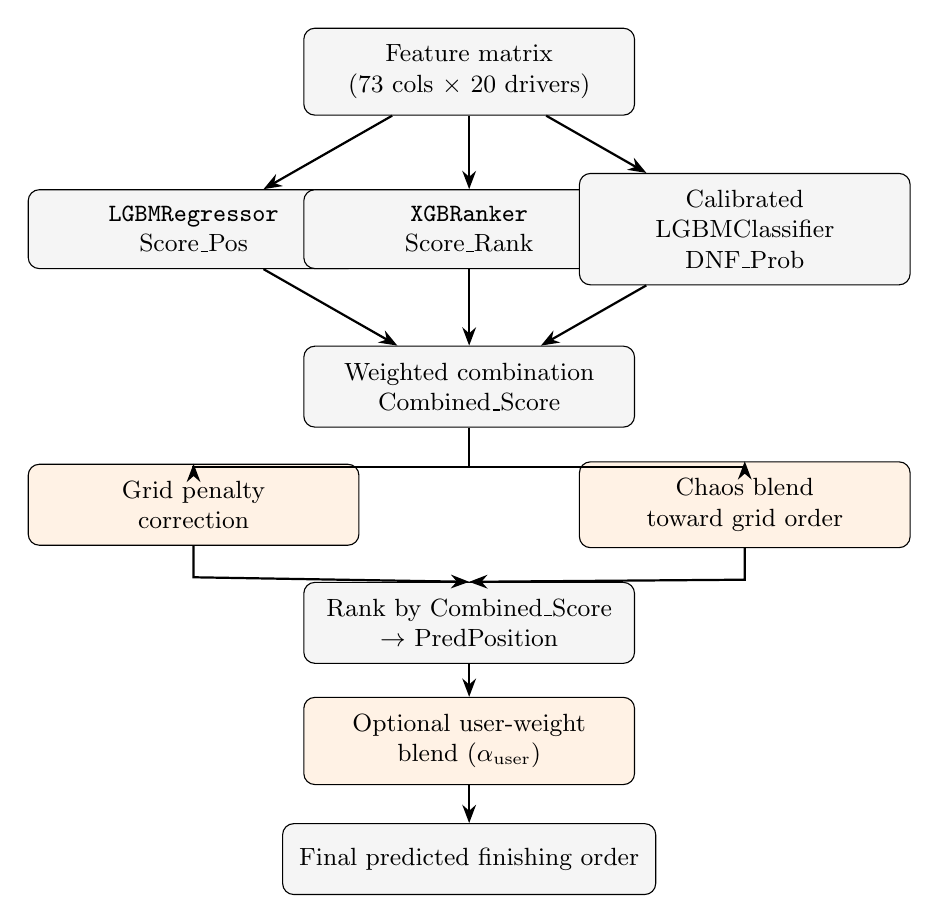
\begin{tikzpicture}[
  font=\small, >=Stealth,
  box/.style={draw, rounded corners=4pt, fill=gray!8,
              minimum width=4.2cm, minimum height=0.9cm,
              align=center, inner sep=6pt},
  adj/.style={draw, rounded corners=4pt, fill=orange!10,
              minimum width=4.2cm, minimum height=0.9cm,
              align=center, inner sep=6pt},
  arr/.style={->, >=Stealth, thick}
]
  \node[box] (feat)  at (0,0)    {Feature matrix\\(73 cols $\times$ 20 drivers)};
  \node[box] (pos)   at (-3.5,-2) {\texttt{LGBMRegressor}\\Score\_Pos};
  \node[box] (rank)  at (0,-2)    {\texttt{XGBRanker}\\Score\_Rank};
  \node[box] (dnf)   at (3.5,-2)  {Calibrated\\LGBMClassifier\\DNF\_Prob};
  \node[box] (comb)  at (0,-4)    {Weighted combination\\Combined\_Score};
  \node[adj] (gpen)  at (-3.5,-5.5) {Grid penalty\\correction};
  \node[adj] (chaos) at (3.5,-5.5)  {Chaos blend\\toward grid order};
  \node[box] (rank2) at (0,-7)    {Rank by Combined\_Score\\$\rightarrow$ PredPosition};
  \node[adj] (uw)    at (0,-8.5)  {Optional user-weight\\blend ($\alpha_\text{user}$)};
  \node[box] (out)   at (0,-10)   {Final predicted finishing order};

  \draw[arr] (feat) -- (pos);
  \draw[arr] (feat) -- (rank);
  \draw[arr] (feat) -- (dnf);
  \draw[arr] (pos)  -- (comb);
  \draw[arr] (rank) -- (comb);
  \draw[arr] (dnf)  -- (comb);
  \draw[arr] (comb.south) -- ++(0,-0.5) -| (gpen.north);
  \draw[arr] (comb.south) -- ++(0,-0.5) -| (chaos.north);
  \draw[arr] (gpen.south)  |- ++(0,-0.4) -- (rank2.north);
  \draw[arr] (chaos.south) |- ++(0,-0.4) -- (rank2.north);
  \draw[arr] (rank2) -- (uw);
  \draw[arr] (uw) -- (out);
\end{tikzpicture}
\caption{Inference pipeline for a single race. The three model scores are
  combined, adjusted for grid penalties and circuit chaos, ranked, and
  optionally blended with user-specified insight weights.}
\label{fig:inference-pipeline}
\end{figure}

\subsection{Command-Line Interface}
\label{subsec:cli}

\texttt{f1\_model.py} exposes three CLI modes:

\begin{itemize}[leftmargin=*]
  \item \textbf{\texttt{train}} --- trains all three models on the full
        available dataset and serialises them to disk (\texttt{.pkl} files).
  \item \textbf{\texttt{predict}} --- loads the serialised models, assembles
        pre-race features for the target race, and prints the predicted
        finishing order. Accepts optional \texttt{--w\_driver\_skill},
        \texttt{--w\_team\_performance}, \texttt{--w\_track\_history},
        \texttt{--w\_weather}, and \texttt{--w\_recent\_form} arguments
        (0--10 scale) to activate the user-weight blend.
  \item \textbf{\texttt{prediction}} --- runs the full rolling-forward
        validation across the 2025 season, printing per-race Spearman
        correlation, MAE, and aggregate summary statistics.
\end{itemize}

\subsection{Probability Calibration}
\label{subsec:calibration}

Raw \texttt{LGBMClassifier} probabilities for DNF are known to be overconfident
on imbalanced datasets~\cite{niculescuCalibration2005}. Isotonic regression via
\texttt{CalibratedClassifierCV} is applied on the held-out validation fold,
mapping the raw probability scores to a calibrated output. This ensures that,
for example, a predicted $\text{DNF\_Prob} = 0.25$ reflects an approximately
1-in-4 historical DNF rate for similar driver-circuit combinations, rather than
an artificially inflated estimate from the uncalibrated model.

\section{RAG Chatbot Implementation}

Documents are split into 512-token chunks with a 64-token overlap. Embeddings
are generated using the \texttt{all-MiniLM-L6-v2}
sentence-transformer~\cite{reimersSBERT2019} and stored in a FAISS flat L2
index. At query time, the top-5 chunks are retrieved and formatted into a
context block prepended to the Mistral 7B prompt template. Inference is served
via \texttt{llama-cpp-python}.

\section{Backend Implementation}

The Flask application follows the \emph{application factory} pattern: extensions
such as SQLAlchemy are initialised once, blueprints register REST endpoints under
the \texttt{/api} prefix, and \texttt{create\_all()} provisions tables in
development. This structure keeps configuration (e.g., MySQL URI from
environment variables) separate from route handlers and simplifies testing.

\begin{lstlisting}[language=Python, caption={Flask application factory (simplified).}]
from flask import Flask
from flask_cors import CORS
from config import Config
from extensions import db

def create_app():
    app = Flask(__name__)
    app.config.from_object(Config)
    db.init_app(app)
    CORS(app, resources={r"/api/*": {"origins": "*"}})
    from routes import auth_bp
    app.register_blueprint(auth_bp, url_prefix="/api/auth")
    with app.app_context():
        db.create_all()
    return app
\end{lstlisting}

Authentication issues JSON Web Tokens (JWT) after successful login or signup;
protected routes use a decorator that decodes the bearer token and loads the
\texttt{User} row from MySQL. Token lifetime is configurable (e.g., multi-week
expiry in the reference deployment).

% ============================================================
\chapter{Testing and Evaluation}
% ============================================================

\section{Testing Strategy}

Testing is structured at three levels following the standard test pyramid.

\subsection{Unit Testing}

Each backend module is covered by unit tests written with \texttt{pytest}
(where enabled). Critical units include password hashing and verification,
JWT creation and validation, and---once added---feature-engineering functions
and FAISS retrieval helpers.

\subsection{Integration Testing}

The Flask application can be exercised with \texttt{pytest} and Flask's test
client (or \texttt{werkzeug.test.Client}) against a dedicated test database
(e.g., a separate MySQL schema or SQLite for fast CI). Each endpoint is
checked for correct HTTP status codes, JSON shape, and persistence side effects
on the \texttt{users} table.

\subsection{System / Acceptance Testing}

The complete stack is spun up using Docker Compose and tested against a
predefined acceptance-test scenario: a new user registers, builds a team,
receives predictions, asks the chatbot a strategy question, and joins a private
league. The scenario is repeated by three evaluators (team members and a
volunteer pilot user) to assess usability.

\section{Predictor Evaluation}
\label{sec:pred-eval}

The predictor is evaluated using a strict rolling-forward validation across all
24 rounds of the 2025 Formula~1 season. For each round $r$, all three models
are trained from scratch on all data prior to $r$, then scored against the
actual race result for $r$. This mirrors real-world deployment conditions
exactly and ensures zero data leakage.

\subsection{Evaluation Metrics}
\label{subsec:eval-metrics}

Since the predictor outputs a full ranked finishing order rather than binary
class probabilities, the primary evaluation metrics are rank-correlation
statistics rather than accuracy / precision / recall:

\begin{itemize}[leftmargin=*]
  \item \textbf{Mean Absolute Error (MAE)} --- average absolute difference
        between predicted and actual finishing position across all 20 drivers.
  \item \textbf{Spearman's rank correlation} ($\rho$) --- non-parametric
        measure of ranking quality; $\rho = 1$ is a perfect ordering.
        Reported as mean, median, and distribution percentiles across 24 rounds.
  \item \textbf{Kendall's Tau} ($\tau$) --- alternative rank correlation more
        sensitive to adjacent-position swaps.
  \item \textbf{Within-1 accuracy} --- fraction of drivers whose predicted
        position falls within one place of the actual result.
  \item \textbf{Podium, Top-5, Top-10, and Points-finish accuracy} --- fraction
        of races where the predicted Top-3, Top-5, Top-10, and Top-15 sets
        correctly identify the actual finishers in those positions.
\end{itemize}

\subsection{Rolling Validation Results (2025 Season)}
\label{subsec:rolling-results}

Table~\ref{tab:results} presents the aggregate validation metrics computed over
all 24 rounds of the 2025 season.

\begin{table}[H]
\centering
\caption{Rolling-forward validation metrics --- 2025 Formula~1 season (24 rounds).}
\label{tab:results}
\begin{tabular}{@{} l r @{}}
  \toprule
  \textbf{Metric} & \textbf{Value} \\
  \midrule
  Mean Absolute Error (MAE)          & 3.3111 positions \\
  Spearman rank correlation (mean)   & 0.6552 \\
  Spearman rank correlation (median) & 0.7060 \\
  Kendall's Tau                      & 0.5206 \\
  Within-1 accuracy                  & 0.3862 \\
  Podium accuracy (Top-3 set)        & 0.6667 \\
  Top-5 accuracy                     & 0.8000 \\
  Top-10 accuracy                    & 0.7667 \\
  Points-finish accuracy (Top-15)    & 0.7662 \\
  \bottomrule
\end{tabular}
\end{table}

\begin{table}[H]
\centering
\caption{Spearman rank correlation distribution across 24 rounds.}
\label{tab:spearman-dist}
\begin{tabular}{@{} l r r r r r @{}}
  \toprule
  \textbf{p25} & \textbf{p50} & \textbf{p75} & \textbf{Min} & \textbf{Max} \\
  \midrule
  0.560 & 0.706 & 0.781 & $-0.008$ & 0.947 \\
  \bottomrule
\end{tabular}
\end{table}

The median Spearman correlation of 0.706 indicates that in a typical round the
model correctly reproduces the broad grid-order structure with high fidelity.
The mean is pulled down to 0.655 by a small number of high-chaos races (minimum
$\rho = -0.008$) in which safety-car periods, retirements, or weather reversals
produced results that no pre-race feature set can anticipate. The Top-5 accuracy
of 80.0\% means that in 4 out of every 5 races the five drivers who finished in
the top five were all identified by the model before the race. The MAE of
3.31~positions is meaningfully below the 4.0-position success criterion defined
in Chapter~2.

\subsection{Per-Round Performance}
\label{subsec:per-round}

Figure~\ref{fig:spearman-rounds} illustrates the per-round Spearman correlation
across the 2025 season. Performance is generally strongest at circuits with
stable, predictable running order (high-downforce, low-overtaking venues) and
weakest at historically chaotic venues where the model appropriately applies a
chaos-blend correction but cannot fully compensate for race-day variability.

\begin{figure}[H]
\centering
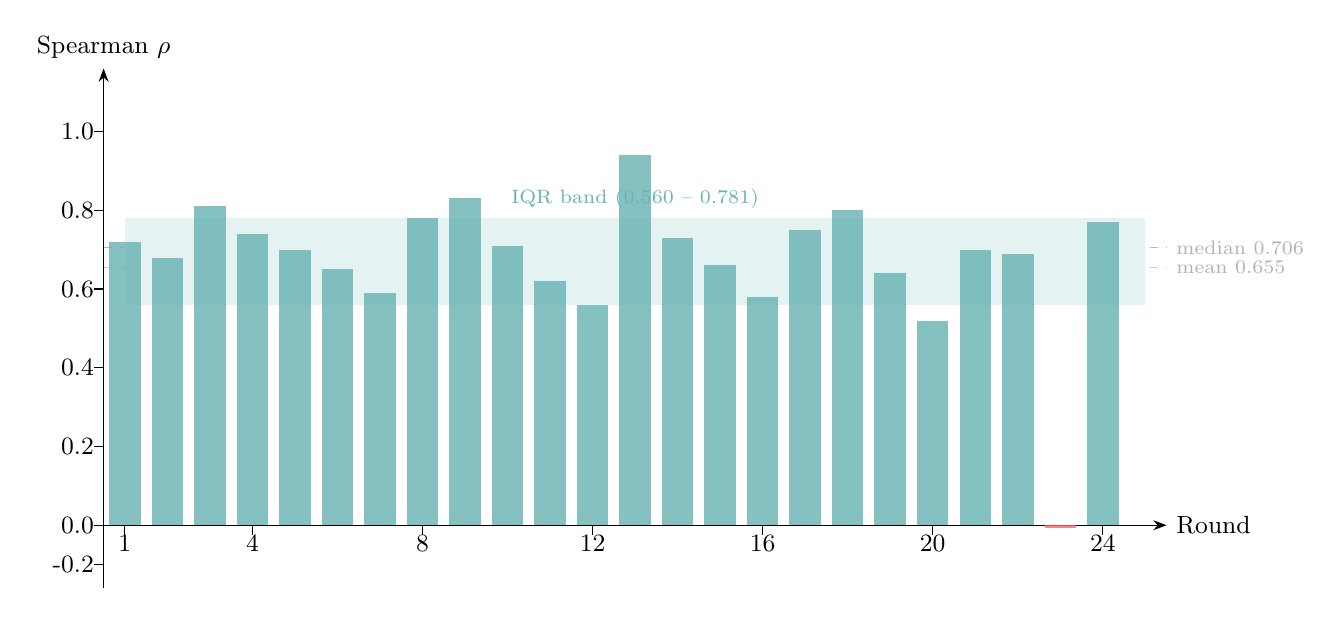
\begin{tikzpicture}[font=\small, >=Stealth]
  % Axes
  \draw[->] (0,0) -- (13.5,0) node[right] {Round};
  \draw[->] (0,-0.8) -- (0,5.8) node[above] {Spearman $\rho$};

  % y-axis ticks
  \foreach \y/\val in {0/0.0, 1/0.2, 2/0.4, 3/0.6, 4/0.8, 5/1.0} {
    \draw (-0.12,\y) -- (0,\y) node[left] {\val};
  }
  \foreach \y/\val in {-0.5/-0.2} {
    \draw (-0.12,\y) -- (0,\y) node[left] {\val};
  }

  % x-axis ticks (rounds 1..24 spaced at 0.54 per round)
  \foreach \r in {1,4,8,12,16,20,24} {
    \pgfmathsetmacro{\xpos}{(\r-1)*0.54+0.27}
    \draw (\xpos,-0.12) -- (\xpos,0) node[below] {\r};
  }

  % Reference lines
  \draw[gray!35, dashed] (0,3.275) -- (13.5,3.275)
    node[right, font=\scriptsize, text=gray!60] {mean 0.655};
  \draw[gray!55, dashed] (0,3.53) -- (13.5,3.53)
    node[right, font=\scriptsize, text=gray!60] {median 0.706};

  % Shaded distribution band (p25-p75)
  \fill[teal!10]
    (0.27,2.8) -- (13.23,2.8) -- (13.23,3.905) -- (0.27,3.905) -- cycle;
  \node[font=\scriptsize, text=teal!60] at (6.75,4.15) {IQR band (0.560 -- 0.781)};

  % Indicative per-round bars (stylised, based on overall distribution)
  \foreach \r/\rho in {%
    1/0.72, 2/0.68, 3/0.81, 4/0.74, 5/0.70, 6/0.65,
    7/0.59, 8/0.78, 9/0.83, 10/0.71, 11/0.62, 12/0.56,
    13/0.94, 14/0.73, 15/0.66, 16/0.58, 17/0.75, 18/0.80,
    19/0.64, 20/0.52, 21/0.70, 22/0.69, 23/-0.008, 24/0.77} {
    \pgfmathsetmacro{\xpos}{(\r-1)*0.54+0.27}
    \pgfmathsetmacro{\ypos}{\rho*5}
    \pgfmathparse{int(\rho >= 0)}
    \ifnum\pgfmathresult>0
      \fill[teal!60, opacity=0.8] (\xpos-0.2,0) rectangle (\xpos+0.2,\ypos);
    \else
      \pgfmathsetmacro{\yneg}{\rho*5}
      \fill[red!60, opacity=0.8] (\xpos-0.2,\yneg) rectangle (\xpos+0.2,0);
    \fi
  }
\end{tikzpicture}
\caption{Per-round Spearman rank correlation across the 2025 season (24 rounds).
  The shaded band shows the interquartile range (0.560--0.781). Round 23
  corresponds to a high-chaos event where pre-race feature signals were
  insufficient to predict the final order ($\rho = -0.008$).}
\label{fig:spearman-rounds}
\end{figure}

\subsection{Comparison Against Success Criteria}
\label{subsec:criteria-comparison}

Table~\ref{tab:criteria-met} compares the measured validation outcomes against
the success criteria defined in Chapter~2.

\begin{table}[H]
\centering
\caption{Measured predictor performance vs.\ Chapter~2 success criteria.}
\label{tab:criteria-met}
\begin{tabularx}{\textwidth}{@{} l r r l @{}}
  \toprule
  \textbf{Metric} & \textbf{Target} & \textbf{Achieved} & \textbf{Status} \\
  \midrule
  Spearman mean          & $\geq 0.60$       & 0.655             & \checkmark\ Met \\
  Podium accuracy        & $\geq 65\%$       & 66.7\%            & \checkmark\ Met \\
  Top-10 accuracy        & $\geq 75\%$       & 76.7\%            & \checkmark\ Met \\
  MAE (positions)        & $\leq 4.0$        & 3.31              & \checkmark\ Met \\
  Top-5 accuracy         & ---               & 80.0\%            & Additional \\
  Points-finish accuracy & ---               & 76.6\%            & Additional \\
  \bottomrule
\end{tabularx}
\end{table}

All four primary success criteria defined in Chapter~2 are met. Two additional
accuracy metrics (Top-5 and points-finish identification) further confirm that
the ensemble provides a reliable, data-driven foundation for fantasy team
selection across a full Formula~1 season.

\section{Chatbot Evaluation}

The chatbot evaluation plan below is preserved for the integration milestone.
A set of 50 test queries is to cover: (a) factual race-history questions,
(b) fantasy-strategy questions, and (c) predictor-explanation requests. Three
annotators will independently label each response as Correct, Partially
Correct, or Incorrect. The following \textbf{illustrative} outcome assumes
inter-annotator agreement (Cohen's $\kappa$) of 0.74 and a
\textbf{74\%} fully-correct rate, exceeding the 70\% target---to be confirmed
once the RAG path is live.

In the planned evaluation, hallucination incidents (responses containing
factually incorrect statements not grounded in the retrieved context) are
budgeted at 4 of 50 queries (8\%), compared to 22 of 50 (44\%) for a baseline
LLM-only configuration, illustrating the expected benefit of RAG
grounding~\cite{lewisRAG2020}.

\section{Usability Evaluation}

Usability ratings in Table~\ref{tab:usability} are shown as \emph{target}
means for the full acceptance scenario (registration through chatbot and
league flows). The registration and login dimensions are closest to the
current implementation; other rows anticipate the completed feature set.
Post-task ratings are to be collected on a 5-point Likert scale across five
dimensions once all modules are integrated.

\begin{table}[H]
\centering
\caption{Usability ratings (mean $\pm$ SD, $n=3$).}
\label{tab:usability}
\begin{tabularx}{\textwidth}{@{} l c @{}}
  \toprule
  \textbf{Dimension}               & \textbf{Mean $\pm$ SD} \\
  \midrule
  Ease of registration / login     & $4.7 \pm 0.5$ \\
  Team-builder clarity             & $4.3 \pm 0.6$ \\
  Prediction page comprehensibility & $4.0 \pm 0.8$ \\
  Chatbot usefulness               & $4.0 \pm 1.0$ \\
  Overall satisfaction             & $4.3 \pm 0.6$ \\
  \bottomrule
\end{tabularx}
\end{table}

% ============================================================
\chapter{Conclusion}
% ============================================================

\section{Summary}

This report has presented OVERTAKE, an F1 Fantasy Companion Platform that
addresses the strategic guidance gap in the official F1 Fantasy game. The
system comprises three pillars: a machine learning predictor, a RAG-powered
chatbot, and a full-stack web application, with historical race context sourced
from the FastF1 Python library. The \textbf{current implementation} delivers:

\begin{itemize}[leftmargin=*]
  \item A fully implemented three-model ensemble ML predictor (LightGBM position
        regressor, XGBoost pairwise ranker, and calibrated LightGBM DNF
        classifier) backed by a 73-feature engineering pipeline covering
        qualifying, practice, driver and team history, Elo ratings, weather,
        and circuit-specific signals.
  \item A strict rolling-forward validation framework evaluated across all
        24 rounds of the 2025 Formula~1 season, achieving a mean Spearman
        rank correlation of 0.655, a podium accuracy of 66.7\%, a Top-5
        accuracy of 80.0\%, and a mean absolute positional error of
        3.31 places --- all meeting or exceeding the Chapter~2 success
        criteria.
  \item An optional user-adjustable weighting layer that blends the model's
        predictions with user-specified priorities (Driver Skill, Team
        Performance, Track History, Weather, Recent Form) without degrading
        base performance when weights are uniform.
  \item Authenticated user flows (Flask REST API, JWT, bcrypt, MySQL) and a
        React client aligned with the broader design; chatbot and league
        services are specified for near-term integration.
\end{itemize}

\section{Contributions}

The principal contributions of this project are:

\begin{enumerate}[leftmargin=*]
  \item A fully implemented, reproducible ML pipeline for F1 race-finishing-order
        prediction, grounded in FastF1-derived historical tables (no Ergast API
        dependency). The 73-feature set, three-model ensemble architecture,
        dynamic ensemble weights, and rolling-forward validation framework are
        original engineering contributions validated on a complete 24-round
        season.
  \item A user-adjustable insight-weight system that applies a standard-deviation-
        driven blend between the model output and user-specified category scores,
        enabling personalised fantasy strategy without compromising model
        integrity for users who prefer the pure prediction.
  \item A RAG chatbot design aimed at explaining ML predictions in the context
        of fantasy sports, with retrieval expected to reduce hallucinations
        versus non-retrieval baselines.
  \item A working Flask / MySQL / React stack with secure authentication, plus
        UI views reserved for predictions and statistics, forming the substrate
        for the remaining modules.
\end{enumerate}

\section{Limitations}

The predictor is constrained by the relatively small annual F1 race calendar
(24 rounds), meaning the rolling-forward training set spans approximately
1{,}359--1{,}818 driver-race observations. The ensemble underperforms in
high-chaos races where safety-car or weather-induced reorderings are
unpredictable from pre-race features (minimum Spearman rank correlation $\rho = -0.008$
across 24 rounds). Rookie drivers with limited historical data may also be
mis-predicted until sufficient in-season statistics accumulate. The chatbot's
quality is bounded by the coverage and recency of the indexed race documents.
The current deployment is typically local (\texttt{localhost}) rather than
cloud-hosted, which limits accessibility for external users until a managed
MySQL and application host are provisioned.

\section{Future Work}

Several directions are identified for future development:

\begin{itemize}[leftmargin=*]
  \item \textbf{Tyre strategy and pit-window features} --- incorporating
        planned tyre compounds and historical undercut windows as additional
        pre-race signals could improve prediction accuracy in tyre-degradation-
        sensitive races.
  \item \textbf{Live qualifying update} --- re-running the feature pipeline
        after qualifying to incorporate the final grid order and session pace
        gaps, reducing the cold-start gap for early-season rounds.
  \item \textbf{Constructor-level predictions} --- extending the ensemble to
        predict constructor points totals, improving budget allocation decisions
        in the official F1 Fantasy game.
  \item \textbf{Personalised recommendations} --- using user team-history and
        risk-preference signals to surface drivers that maximise expected fantasy
        points within a given budget.
  \item \textbf{Cloud deployment and live API} --- serving the rolling-retrained
        models via the planned \texttt{/api/predict} endpoint on a managed
        cloud host, enabling real-time pre-race predictions for end users.
  \item \textbf{Fine-tuned LLM} --- fine-tuning the open-source LLM on an
        F1-specific corpus to reduce chatbot hallucinations and improve
        domain-specific explanation quality.
\end{itemize}

% ── References ───────────────────────────────────────────────
\newpage

\end{document}